\section{\texorpdfstring{\emph{How Pythagorean Quintuplets, Sextuplets, and Octuplets Crack Composite Numbers Wide Open}}{How Pythagorean Quintuplets, Sextuplets, and Octuplets Crack Composite Numbers Wide Open}}\label{ch6-how-pythagorean-quintuplets-sextuplets-and-octuplets-crack-composite-numbers-wide-open}



\section{The Locksmith's Dilemma}\label{ch6-the-locksmiths-dilemma}

Imagine a safe whose combination lock has not one keyhole, but \emph{seven}. Any single key that fits any single hole will swing the door open. You don't need all seven keys --- you need only \emph{one} that works. The puzzle:

\begin{quote}
\emph{Given a composite number \(N\), how many independent ``keyholes'' can you create from a single equation?}
\end{quote}

By now, you and I are old friends of the Pythagorean equation \(a^2 + b^2 = c^2\). In earlier chapters we learned that it yields one elegant factoring channel: the identity

\[(c - b)(c + b) = a^2,\]

from which \(\gcd(c - b, N)\) may betray a hidden factor of \(N\). One equation, one keyhole, one shot at cracking the safe. Respectable --- but not spectacular.

Here is the question that will occupy us for the rest of this chapter, and it is the kind of question that, once asked, makes you wonder why nobody asked it sooner: \emph{What if we had more terms on the left-hand side?}

Instead of two squares summing to a third, consider three. Or four. Or seven. The equation

\[a_1^2 + a_2^2 + \cdots + a_k^2 = N^2\]

is a higher-dimensional cousin of the Pythagorean relation --- and each of those \(k\) summands on the left, as we shall see, furnishes an independent attempt to pick the lock. The more tumblers, the more chances.

To make this precise, recall the generalized \index{Lorentz form}Lorentz form we met in Chapter 5:

\[Q_{n,1}(\mathbf{v}) = v_0^2 + v_1^2 + \cdots + v_{n-1}^2 - v_n^2.\]

The \emph{null cone} is the set of integer vectors where \(Q_{n,1}(\mathbf{v}) = 0\) --- that is, where

\[\sum_{i=0}^{n-1} v_i^2 = v_n^2.\]

This is nothing but the Pythagorean equation in \(n + 1\) variables, with \(v_n\) playing the role of the hypotenuse. In the classical case, \(n = 2\), the \index{null cone}null cone is our familiar light cone, and its integer points are the \index{Pythagorean triple}Pythagorean triples. But the cone exists in every dimension, and its integer points --- Pythagorean \(k\)-tuples for every \(k\) --- are the keys to our seven-holed lock.

Think of it this way. The spatial components \(v_0, v_1, \ldots, v_{n-1}\) are the \emph{tumblers} of the lock. The hypotenuse \(v_n = N\) is the \emph{door}. Each tumbler offers an independent attempt to pick the lock, because each one yields a different algebraic identity linking the tumbler to the composite we wish to factor. One tumbler might fail --- the GCD might come out as \(1\) or \(N\), revealing nothing. But with seven tumblers, the odds shift dramatically in the lockpicker's favor.


\begin{figure}[htbp]
\centering
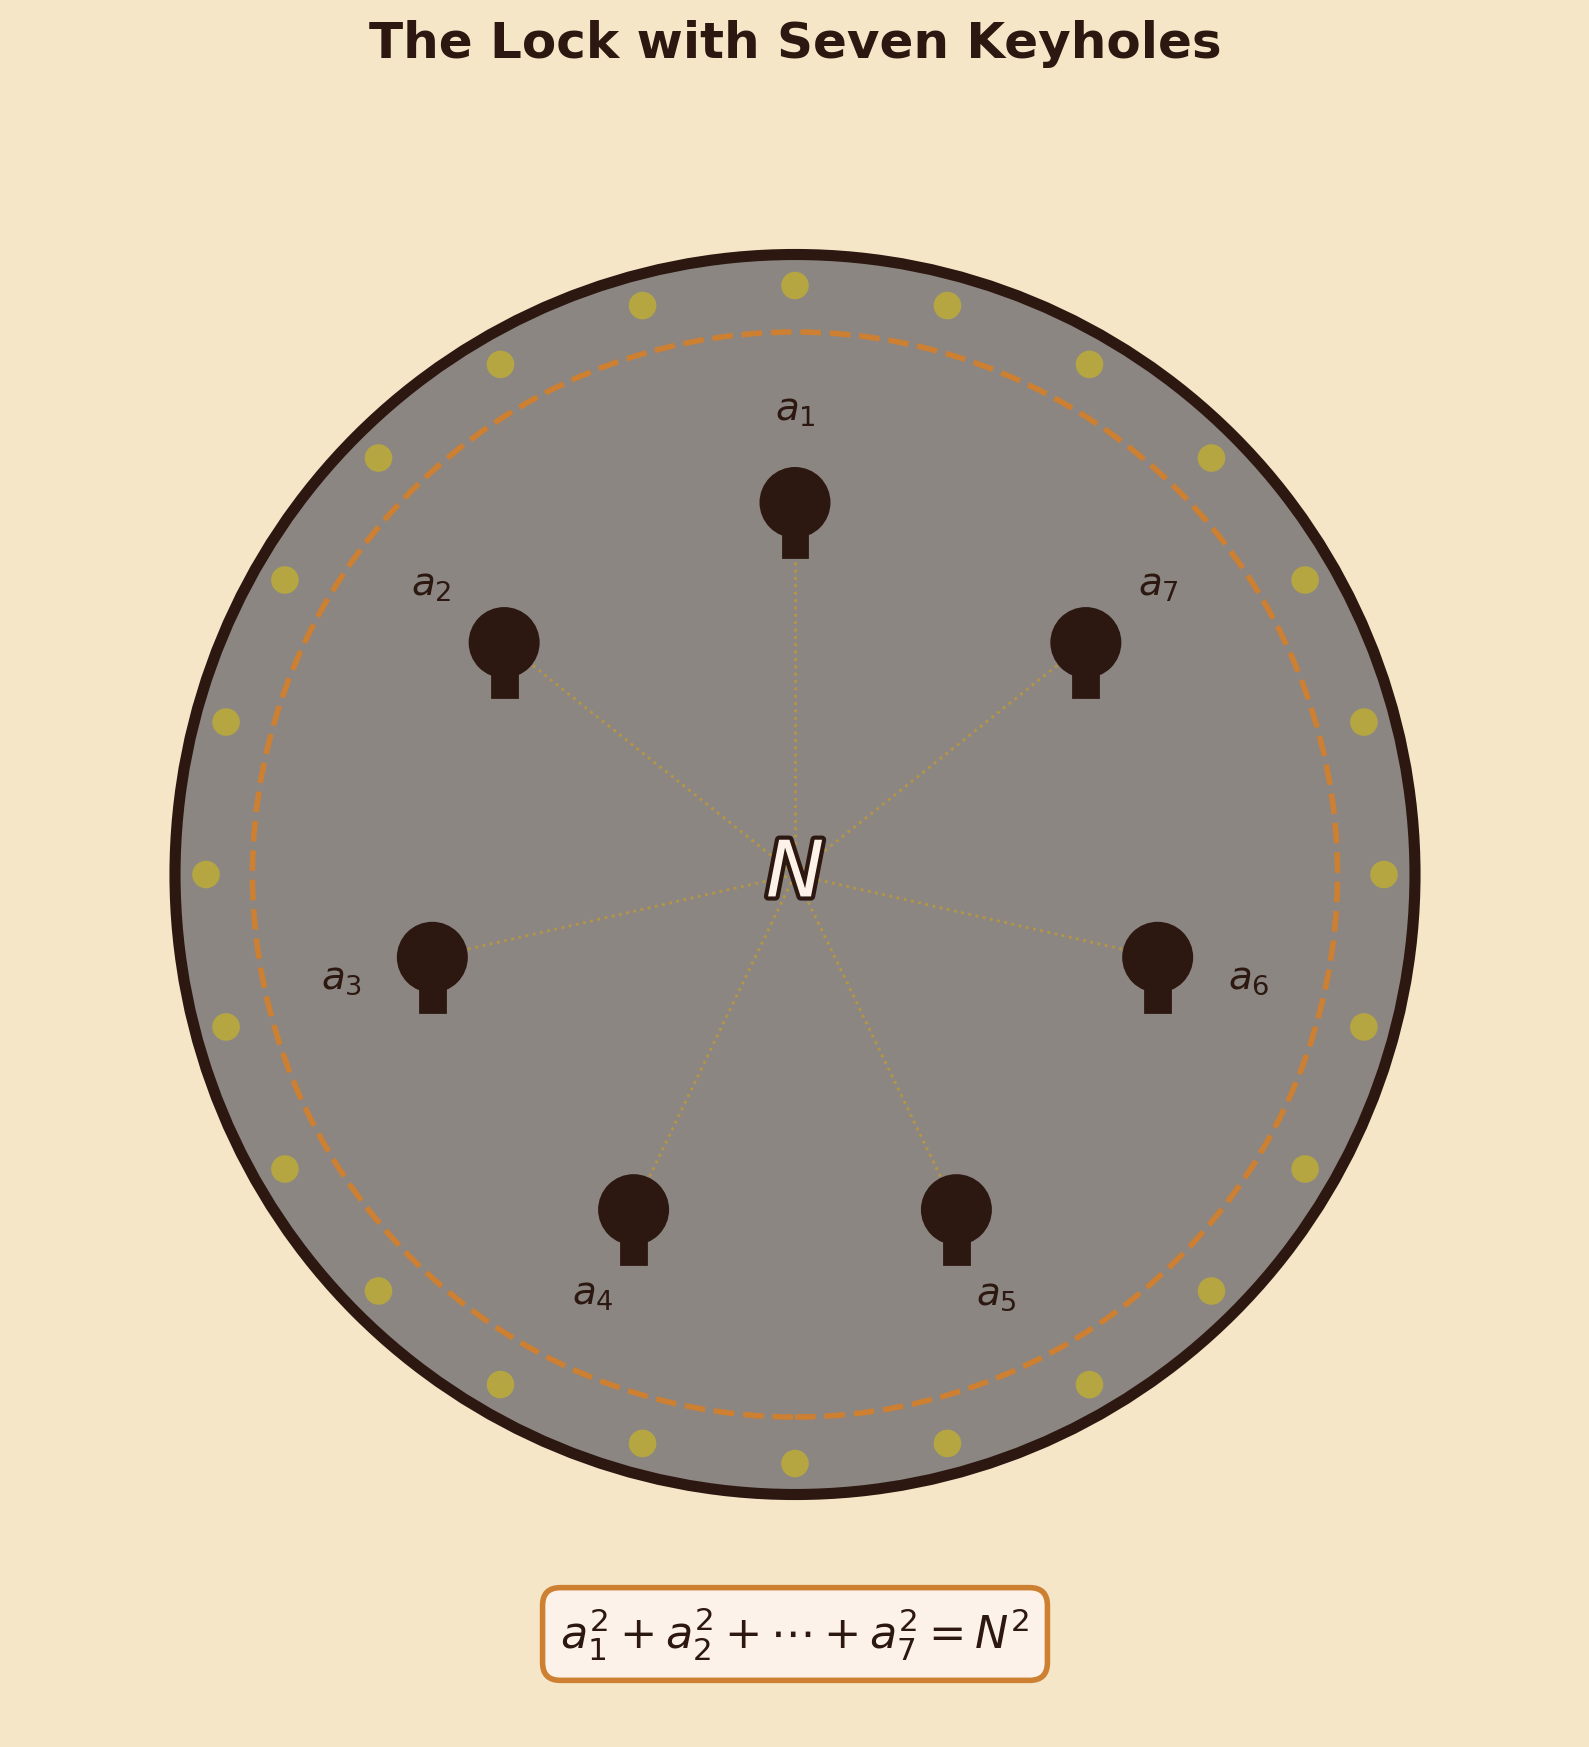
\includegraphics[width=0.82\textwidth]{../Chapter6/images/fig01_vault_seven_keyholes.png}
\end{figure}


A brief historical aside is irresistible here. The \index{quadratic form}quadratic form \(Q_{n,1}\) was introduced by Hermann Minkowski in 1907 to reformulate Einstein's \index{special relativity}special relativity. In physics, the null cone is the path of light --- the boundary between events that can influence each other and those that cannot. In number theory, the very same algebraic object governs the arithmetic of Pythagorean \(k\)-tuples. The null cone in physics tells you what you \emph{can reach}; in number theory, it tells you what you \emph{can factor}. Mathematics, as usual, does not care which question you thought you were asking.



\section{A Menagerie of Pythagorean Creatures}\label{ch6-a-menagerie-of-pythagorean-creatures}

Everyone knows the Pythagorean triple. \(3^2 + 4^2 = 5^2\): three, four, five --- the mascot of every geometry textbook since Euclid. Fewer people have met its four-legged cousin, the Pythagorean \emph{quadruple}: \(1^2 + 2^2 + 2^2 = 3^2\). And almost nobody has encountered the eight-legged beast lurking at the far end of the menagerie. Let us visit the zoo.

A \textbf{Pythagorean quintuplet} is a tuple \((a, b, c, d, e)\) of positive integers satisfying

\[a^2 + b^2 + c^2 + d^2 = e^2.\]

Examples are not hard to find, though they may surprise you with their variety. The smallest is almost comically symmetric: \((1, 1, 1, 1, 2)\), since \(1 + 1 + 1 + 1 = 4 = 2^2\). Then there is the slightly more adventurous \((1, 2, 2, 4, 5)\), since \(1 + 4 + 4 + 16 = 25\). And the lovely \((1, 4, 4, 4, 7)\), since \(1 + 16 + 16 + 16 = 49\). Already a pattern suggests itself: four squares summing to a perfect square is not a rare event. It is, in fact, guaranteed by a theorem we will meet at the end of this chapter.

A \textbf{Pythagorean sextuplet} adds a fifth leg:

\[a^2 + b^2 + c^2 + d^2 + e^2 = f^2.\]

Try \((1, 1, 1, 2, 3, 4)\): we get \(1 + 1 + 1 + 4 + 9 = 16 = 4^2\). Or the more elegant \((1, 1, 3, 3, 4, 6)\): \(1 + 1 + 9 + 9 + 16 = 36 = 6^2\). The world of sextuplets is vast and mostly unexplored by recreational mathematicians --- which is a pity, because it holds treasures.

And then there is the \textbf{Pythagorean octuplet}, the eight-legged octopus of the family:

\[a_1^2 + a_2^2 + a_3^2 + a_4^2 + a_5^2 + a_6^2 + a_7^2 = w^2.\]

Here is a specimen: \((1, 2, 3, 4, 5, 6, 3, 10)\), since \(1 + 4 + 9 + 16 + 25 + 36 + 9 = 100 = 10^2\). The octuplet will be our star performer in this chapter, for reasons that will become clear in Section 3.


\begin{figure}[htbp]
\centering
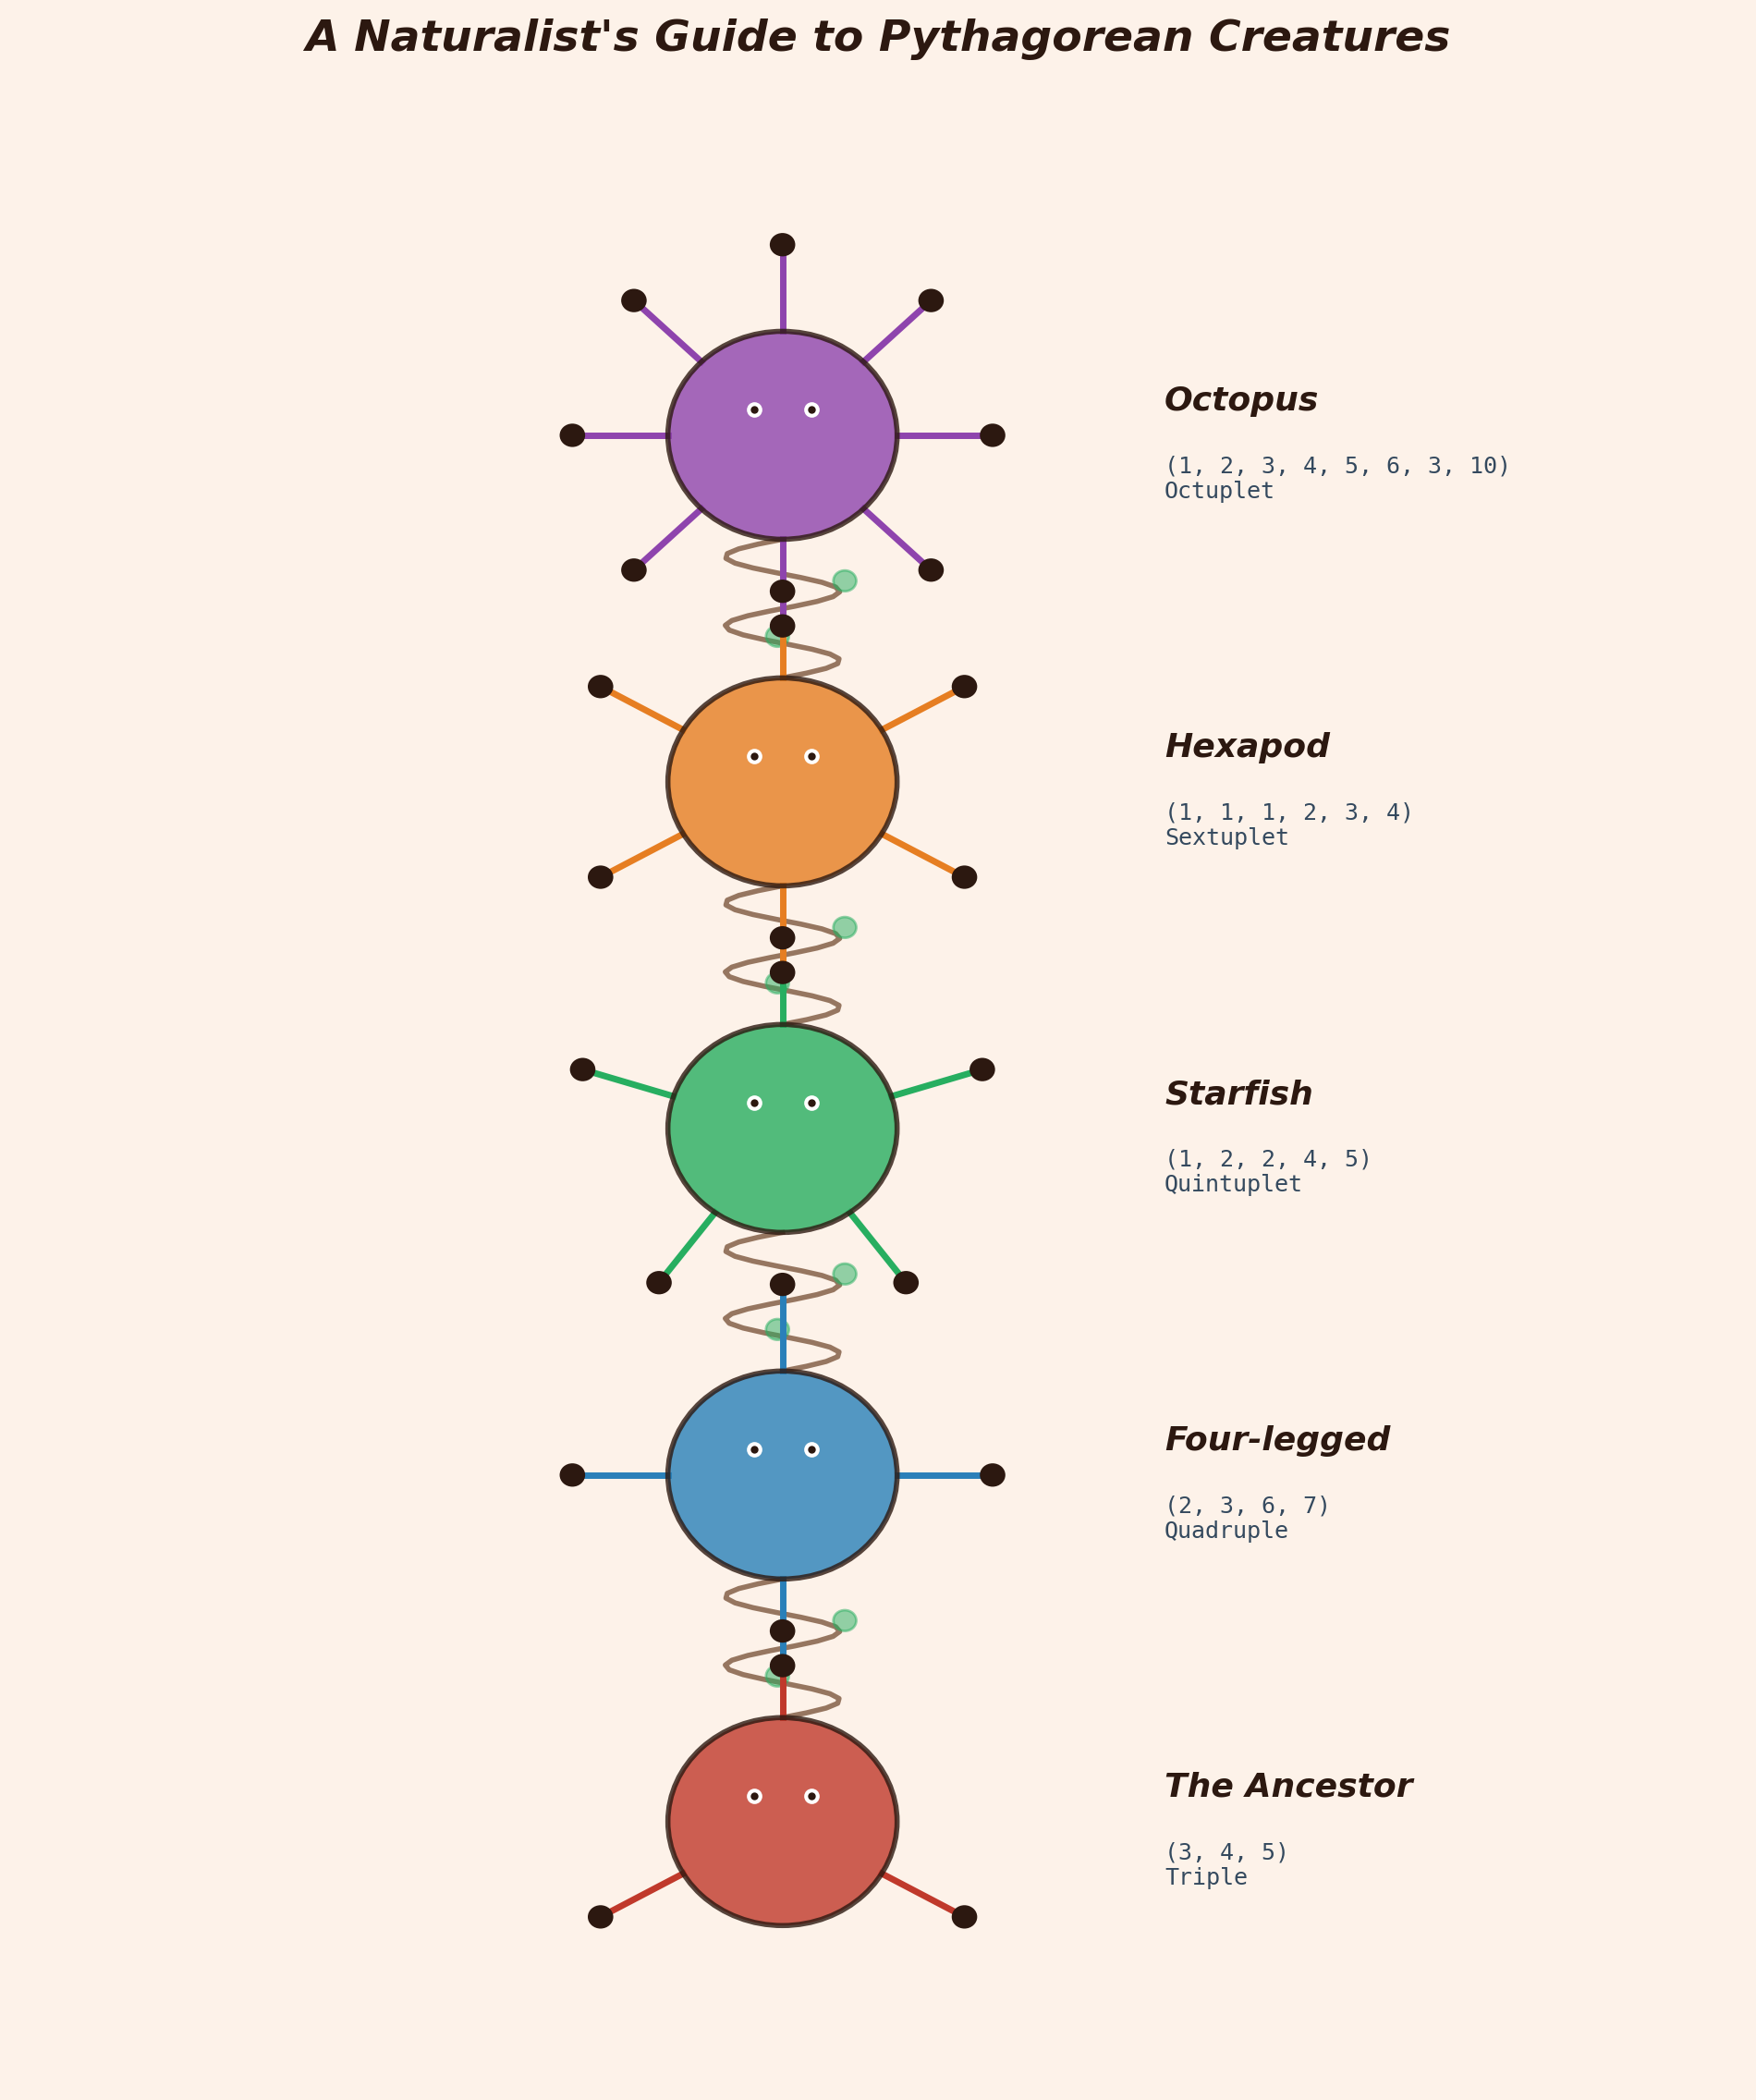
\includegraphics[width=0.82\textwidth]{../Chapter6/images/fig02_phylogenetic_tree.png}
\end{figure}



\begin{figure}[htbp]
\centering
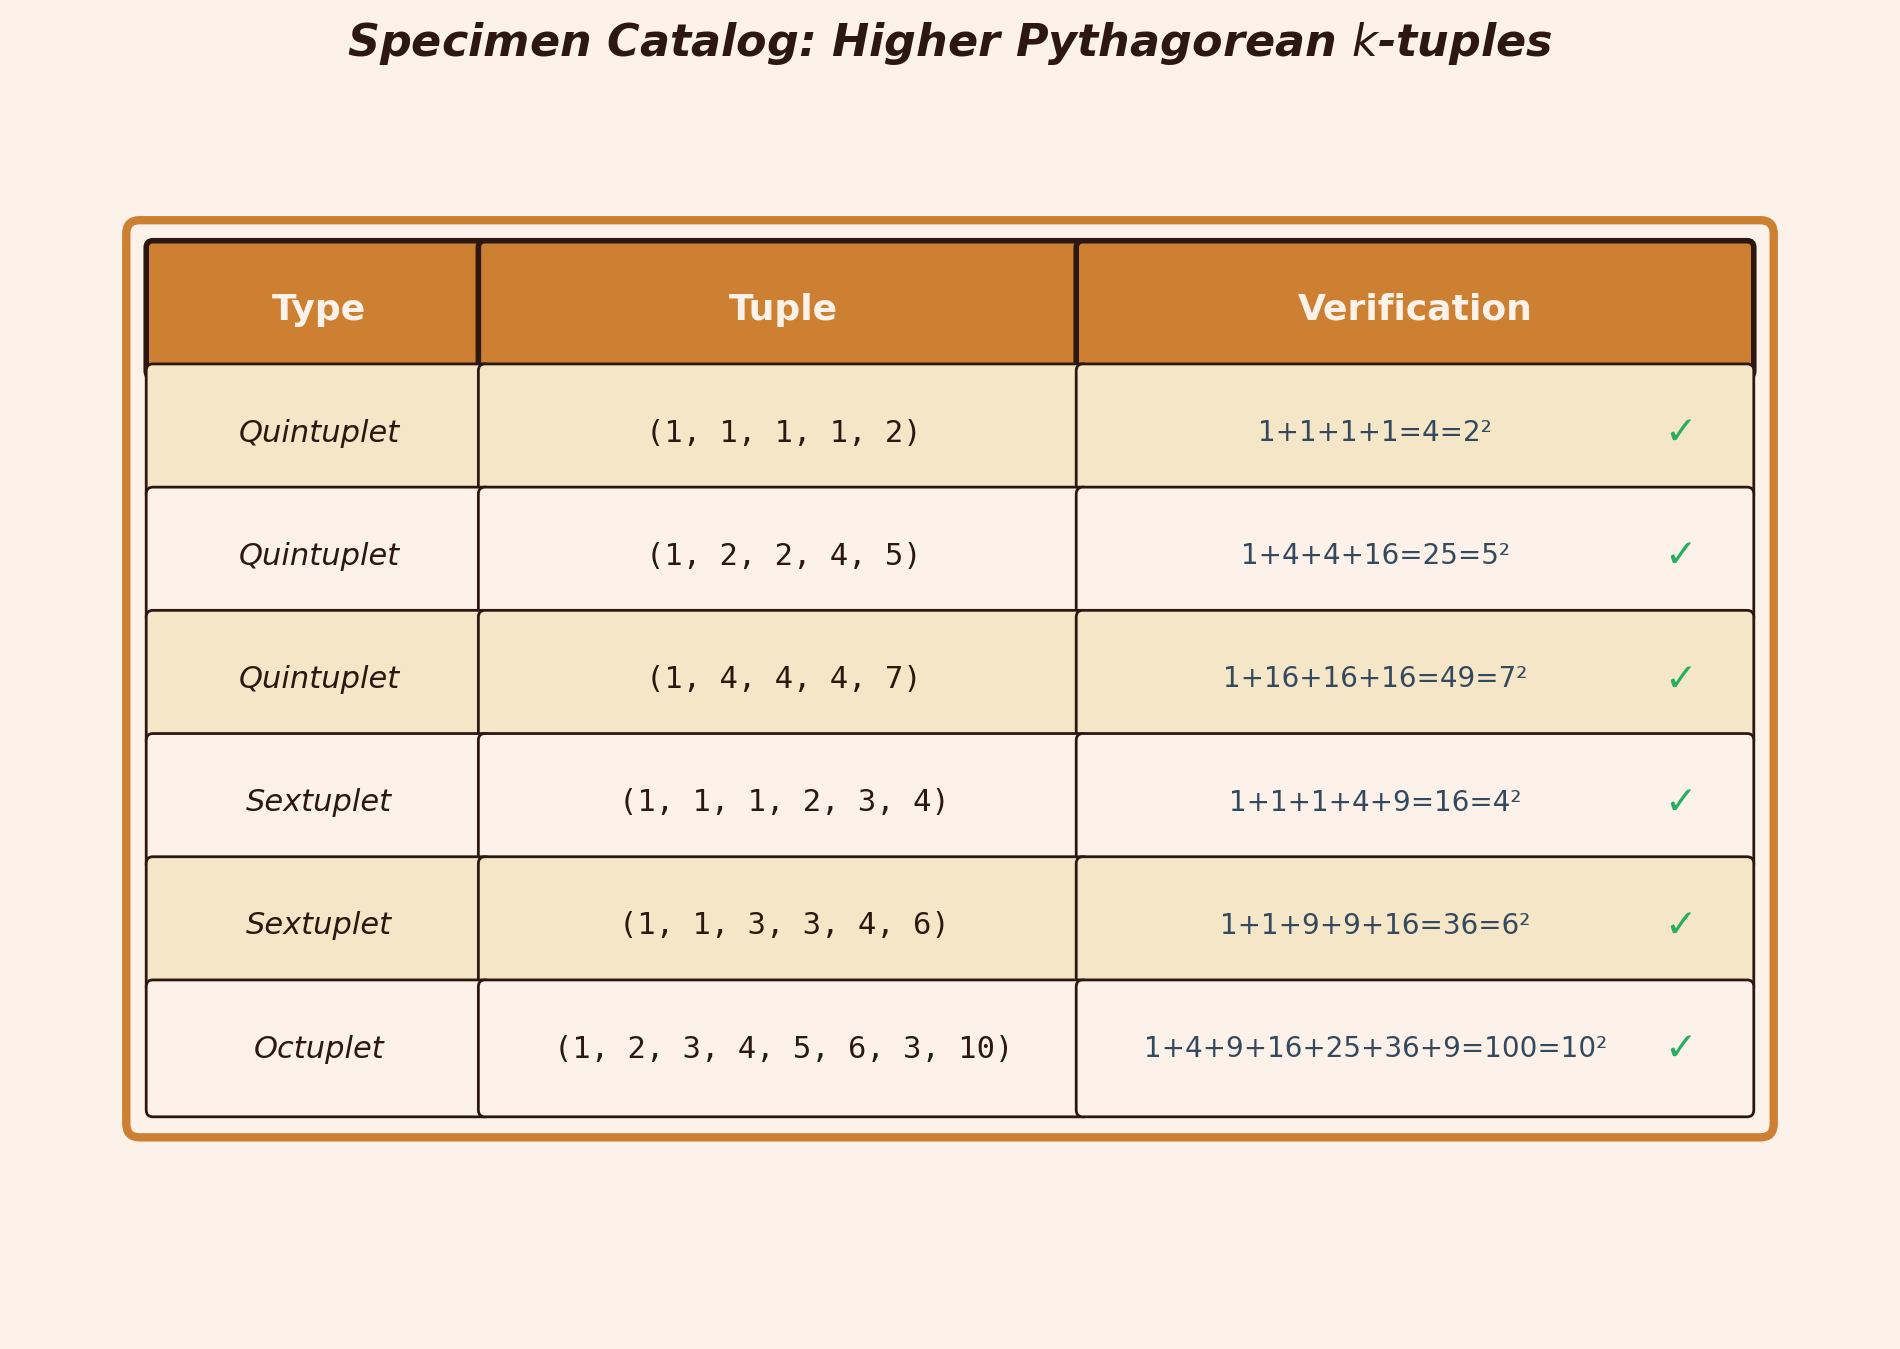
\includegraphics[width=0.82\textwidth]{../Chapter6/images/fig03_specimen_catalog.png}
\end{figure}


\textbf{A puzzle for the reader.} Find a Pythagorean quintuplet \((a, b, c, d, e)\) where all four spatial components \(a, b, c, d\) are \emph{distinct primes}. (Hint: try the smallest primes and check whether \(a^2 + b^2 + c^2 + d^2\) happens to be a perfect square.)

The sums-of-squares problem has a glorious pedigree. Fermat proved that every prime \(p \equiv 1 \pmod{4}\) is a sum of two squares. Lagrange proved that \emph{every} positive integer is a sum of four squares --- a result so beautiful that Lagrange himself, not a man prone to aesthetic rapture, reportedly called it ``one of the most satisfying truths in arithmetic.'' Jacobi went further, giving an exact formula for the number of representations \(r_4(n)\) --- the number of ways to write \(n\) as a sum of four squares (counting signs and order). We are now asking a sharper question: when can \(n\) be a \emph{perfect square}, and what does that structure tell us about its prime factors?



\section{The Multi-Channel Theorem --- One Equation, Many Keys}\label{ch6-the-multi-channel-theorem-one-equation-many-keys}

A classical safecracker gets one try per combination. A quantum safecracker --- the subject of a future chapter --- gets a square-root speedup. But a \emph{Pythagorean} safecracker, working in dimension \(k\), gets \(k - 1\) entirely independent tries from the very same equation. The higher the dimension, the more chances. Let me show you how.

Suppose we have a Pythagorean quadruple --- three spatial components and a hypotenuse:

\[a^2 + b^2 + c^2 = N^2.\]

Focus on the third component \(c\). We can rearrange:

\[(N - c)(N + c) = N^2 - c^2 = a^2 + b^2.\]

This is a difference-of-squares factorization, and the left-hand side is a product of two integers, both of which are closely related to \(N\). In particular, \(N\) divides \((N - c)(N + c) + c^2 - c^2 = N^2\), and so any common factor of \(N - c\) and \(N\) is a factor of \(N\) itself. Therefore:

\[\gcd(N - c, \, N)\]

is a candidate nontrivial factor of \(N\).

But here is the bonanza: we can do the same trick with \(b\):

\[(N - b)(N + b) = a^2 + c^2,\]

and again with \(a\):

\[(N - a)(N + a) = b^2 + c^2.\]

Three spatial components, three independent factoring channels --- three different keys being tried in three different keyholes. If any one of them yields a GCD that is strictly between \(1\) and \(N\), the safe swings open.

Let me state this as a theorem, informally but precisely:

\begin{quote}
\textbf{The Multi-Channel Factor Extraction Theorem.} Let \(a_1^2 + a_2^2 + \cdots + a_{k-1}^2 = N^2\) be a Pythagorean \(k\)-tuple with hypotenuse \(N\). For each spatial component \(a_i\), we have

\[(N - a_i)(N + a_i) = \sum_{j \ne i} a_j^2,\]

and therefore \(\gcd(N - a_i, \, N)\) divides \(N\). If \(1 < \gcd(N - a_i, \, N) < N\) for any \(i\), then \(N\) has a nontrivial factor.
\end{quote}

The proof is immediate: \(\gcd(N - a_i, \, N)\) divides \(N\) by definition of the GCD, and if it is strictly between \(1\) and \(N\), it is neither trivial nor the whole number. But the \emph{power} of the theorem lies not in the proof but in the \emph{multiplicity}: a Pythagorean octuplet with hypotenuse \(N\) provides seven primary channels, one per spatial component. Seven keys, seven keyholes, one equation.

There is also a duality worth noting. Each spatial component yields not one but \emph{two} GCD candidates: the ``minus channel'' \(\gcd(N - a_i, N)\) and the ``plus channel'' \(\gcd(N + a_i, N)\). Both divide \(N\). So a pedantic accountant would count fourteen attempts from a single octuplet --- but since the plus and minus channels from the same component are closely related, we conservatively count seven primary channels.

Let us see the theorem in action.

\textbf{Worked Example --- Cracking \(N = 15\).} Consider the quadruple \((5, 10, 10, 15)\):

\[5^2 + 10^2 + 10^2 = 25 + 100 + 100 = 225 = 15^2. \checkmark\]

Three channels:

\begin{itemize}

\item
  Via \(a = 5\): \(\gcd(15 - 5, 15) = \gcd(10, 15) = 5\). Since \(1 < 5 < 15\) --- \emph{factor found!}
\item
  Via \(b = 10\): \(\gcd(15 - 10, 15) = \gcd(5, 15) = 5\). Again a hit.
\item
  Via \(c = 10\): \(\gcd(15 - 10, 15) = \gcd(5, 15) = 5\). And again.
\end{itemize}

All three channels crack the same factor, \(5\), giving \(15 = 5 \times 3\). In this case, the lock was almost embarrassingly easy --- but note that \emph{any one} of the three channels would have sufficed.

\textbf{Worked Example --- Cracking \(N = 21\).} Consider \((6, 9, 18, 21)\):

\[6^2 + 9^2 + 18^2 = 36 + 81 + 324 = 441 = 21^2. \checkmark\]

Three channels:

\begin{itemize}

\item
  Via \(a = 6\): \(\gcd(21 - 6, 21) = \gcd(15, 21) = 3\). Factor found: \(21 = 3 \times 7\).
\item
  Via \(b = 9\): \(\gcd(21 - 9, 21) = \gcd(12, 21) = 3\). Same factor.
\item
  Via \(c = 18\): \(\gcd(21 - 18, 21) = \gcd(3, 21) = 3\). And again.
\end{itemize}


\begin{figure}[htbp]
\centering
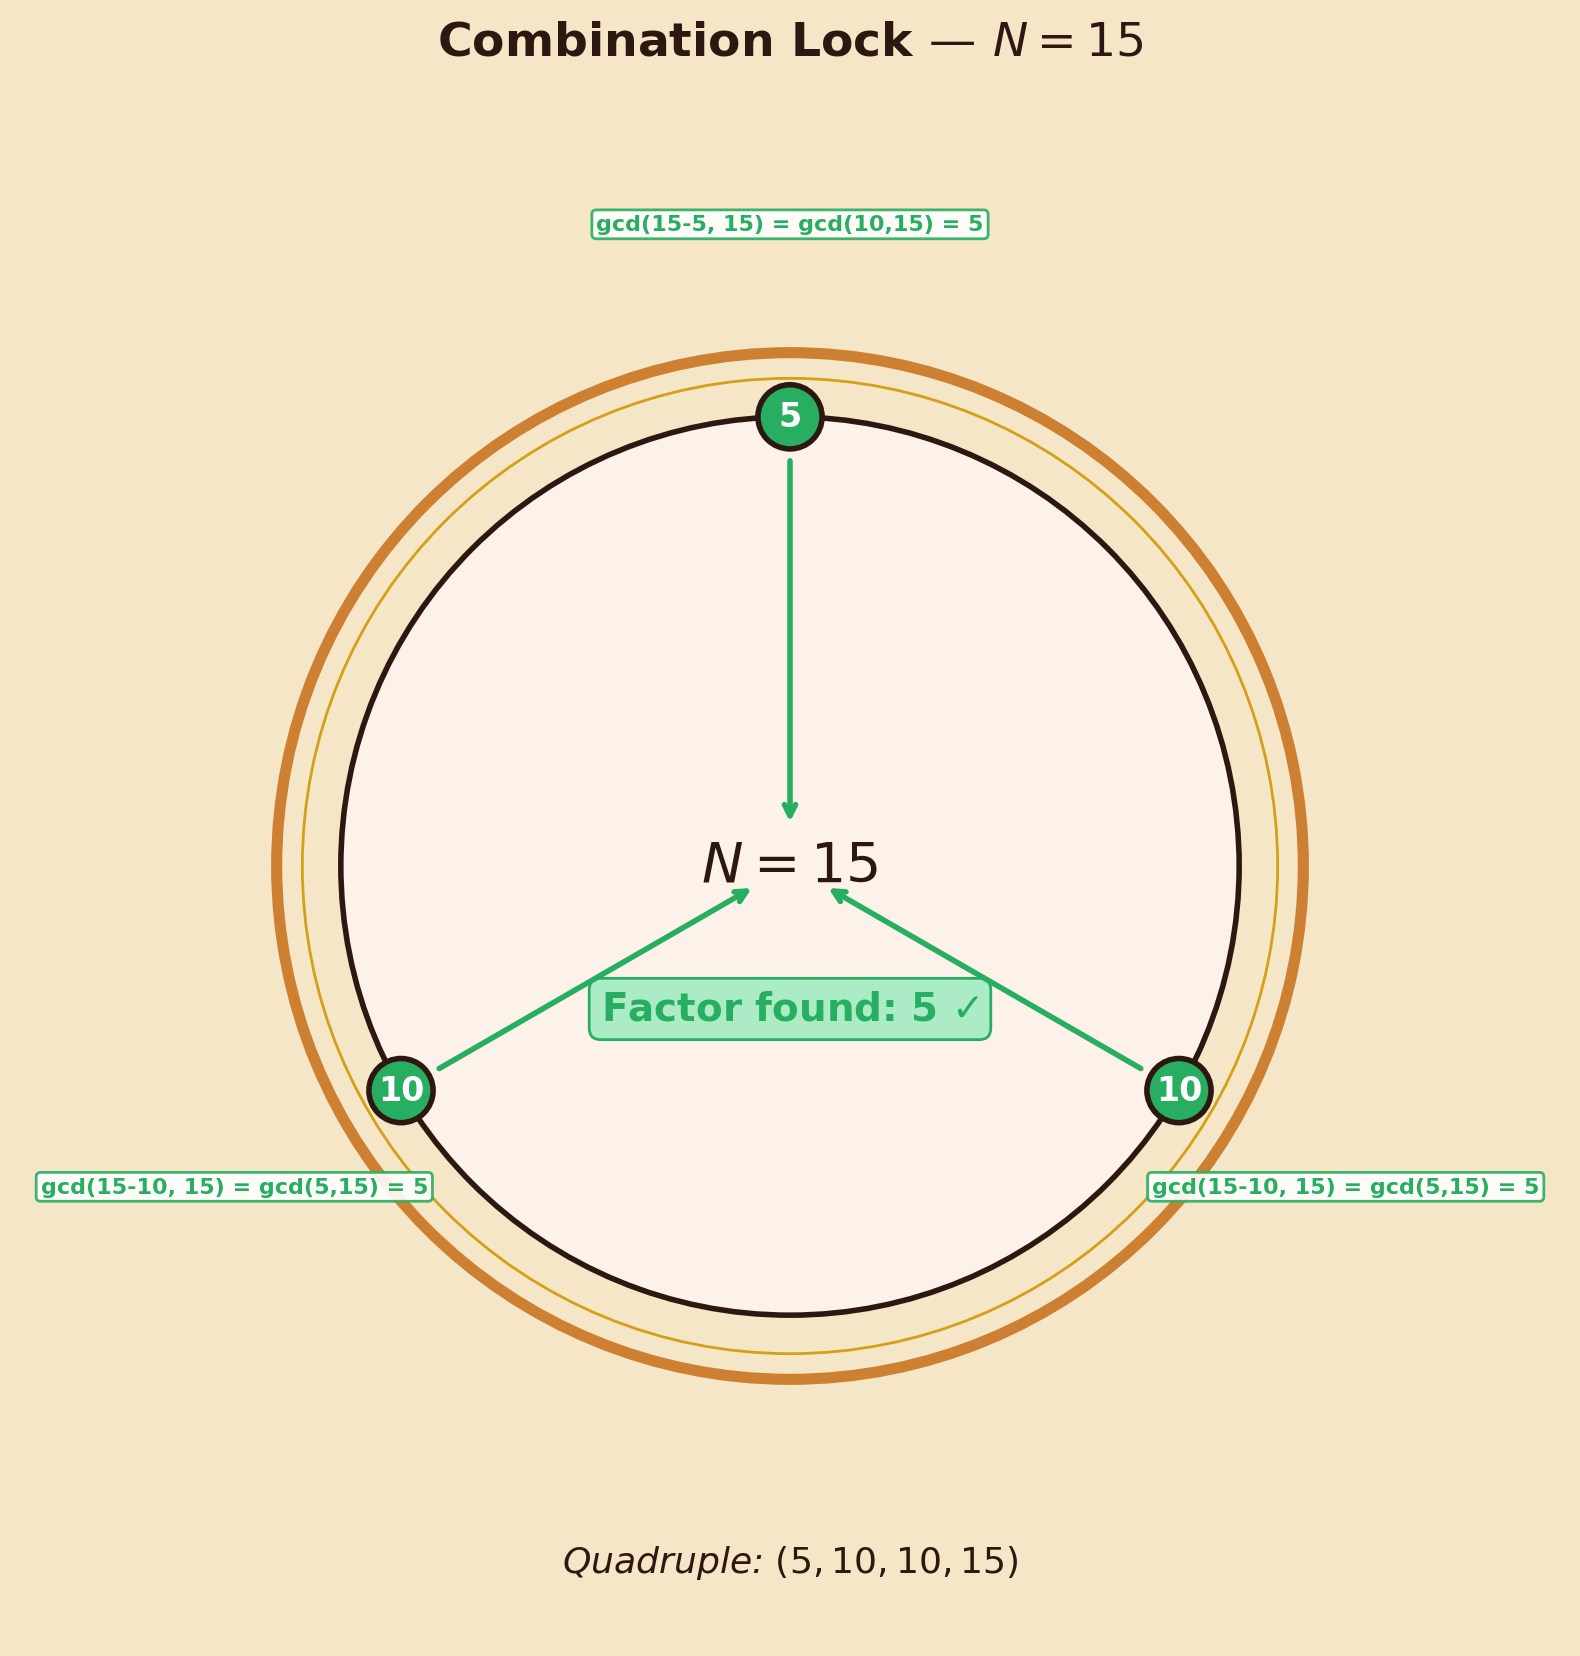
\includegraphics[width=0.82\textwidth]{../Chapter6/images/fig04_lock_N15.png}
\end{figure}



\begin{figure}[htbp]
\centering
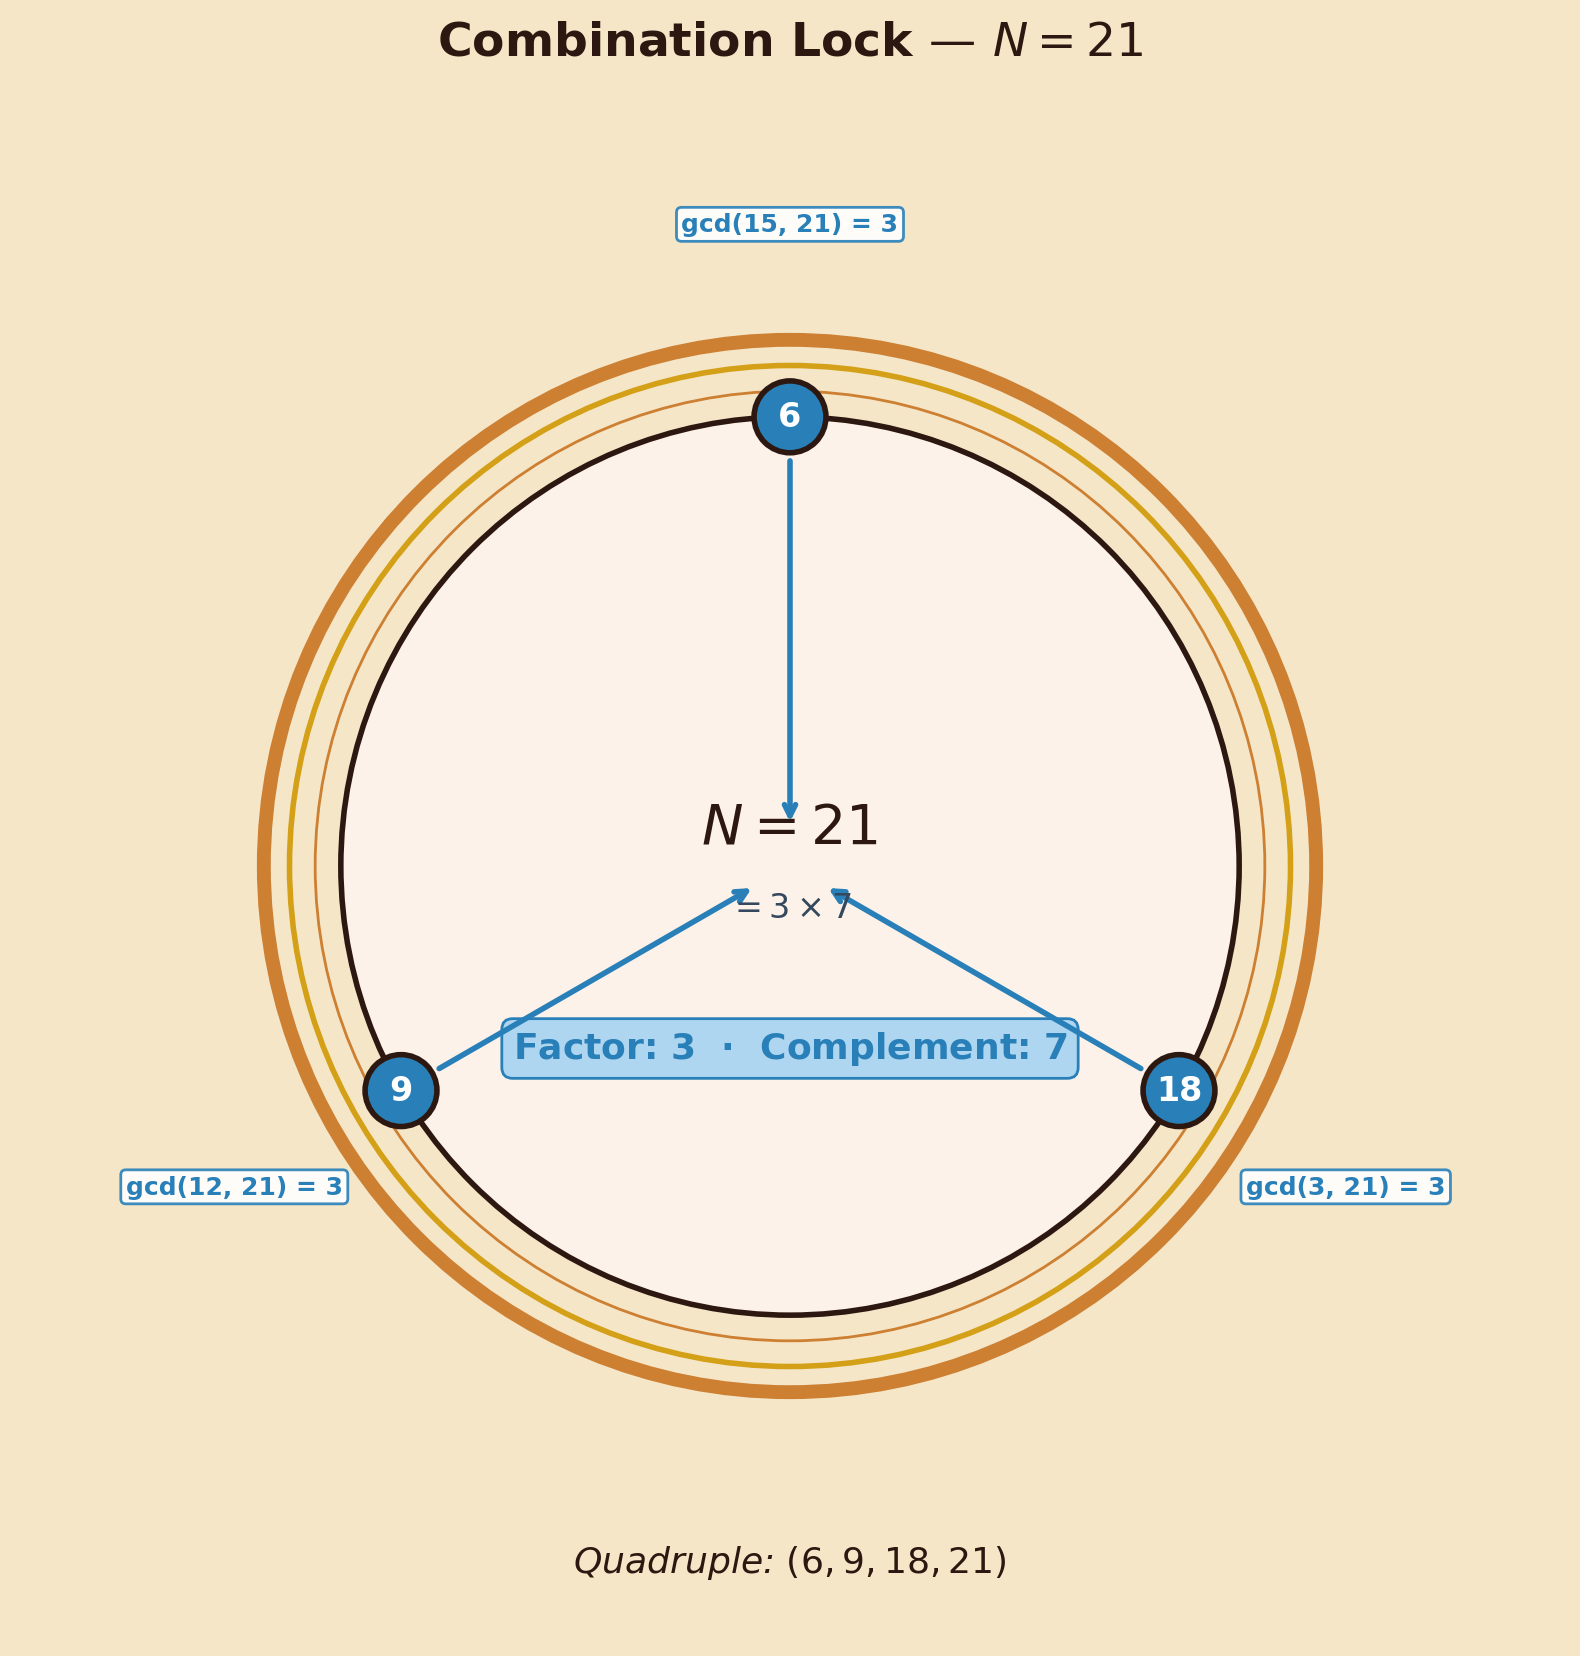
\includegraphics[width=0.82\textwidth]{../Chapter6/images/fig05_lock_N21.png}
\end{figure}




\section{Comparing Tumblers --- The Pairwise Channel Theorem}\label{ch6-comparing-tumblers-the-pairwise-channel-theorem}

But the channels don't stop at the primary ones. Just as a locksmith can learn something by \emph{comparing} two tumblers --- measuring one against another --- the factorer can extract information from \emph{pairs} of spatial components. And for an octuplet, there are \(\binom{7}{2} = 21\) such pairs.

Here is the idea. Given a Pythagorean quadruple \(a^2 + b^2 + c^2 = N^2\), consider the difference of the first two components' squares:

\[a^2 - b^2 = (a - b)(a + b).\]

Now, from the original equation, \(a^2 = N^2 - b^2 - c^2\), so

\[a^2 - b^2 = N^2 - 2b^2 - c^2.\]

The right side is an integer determined by \(N\) and the tuple. The left side factors as \((a - b)(a + b)\). Therefore:

\[\gcd\!\big((a - b)(a + b),\, N\big) = \gcd(a^2 - b^2, \, N)\]

divides \(N\), and if it is nontrivial, we have cracked the safe from a completely different angle --- not by comparing a single tumbler to the door, but by comparing two tumblers \emph{to each other}.

\textbf{The channel census for octuplets.} An octuplet with \(7\) spatial components provides:

\begin{itemize}

\item
  \(7\) \textbf{primary channels} (one per component, as in Section 3).
\item
  \(\binom{7}{2} = 21\) \textbf{pairwise channels} (one per unordered pair of components).
\item
  \textbf{Total: \(28\) independent factoring attempts from a single equation.}
\end{itemize}

Twenty-eight keys from one equation. The classical number theorist, armed with Fermat's original difference-of-squares method, gets essentially \emph{one} channel at a time --- and must search laboriously for a suitable representation. The multi-channel approach converts a single Pythagorean representation into a whole \emph{bundle} of simultaneous attacks.


\begin{figure}[htbp]
\centering
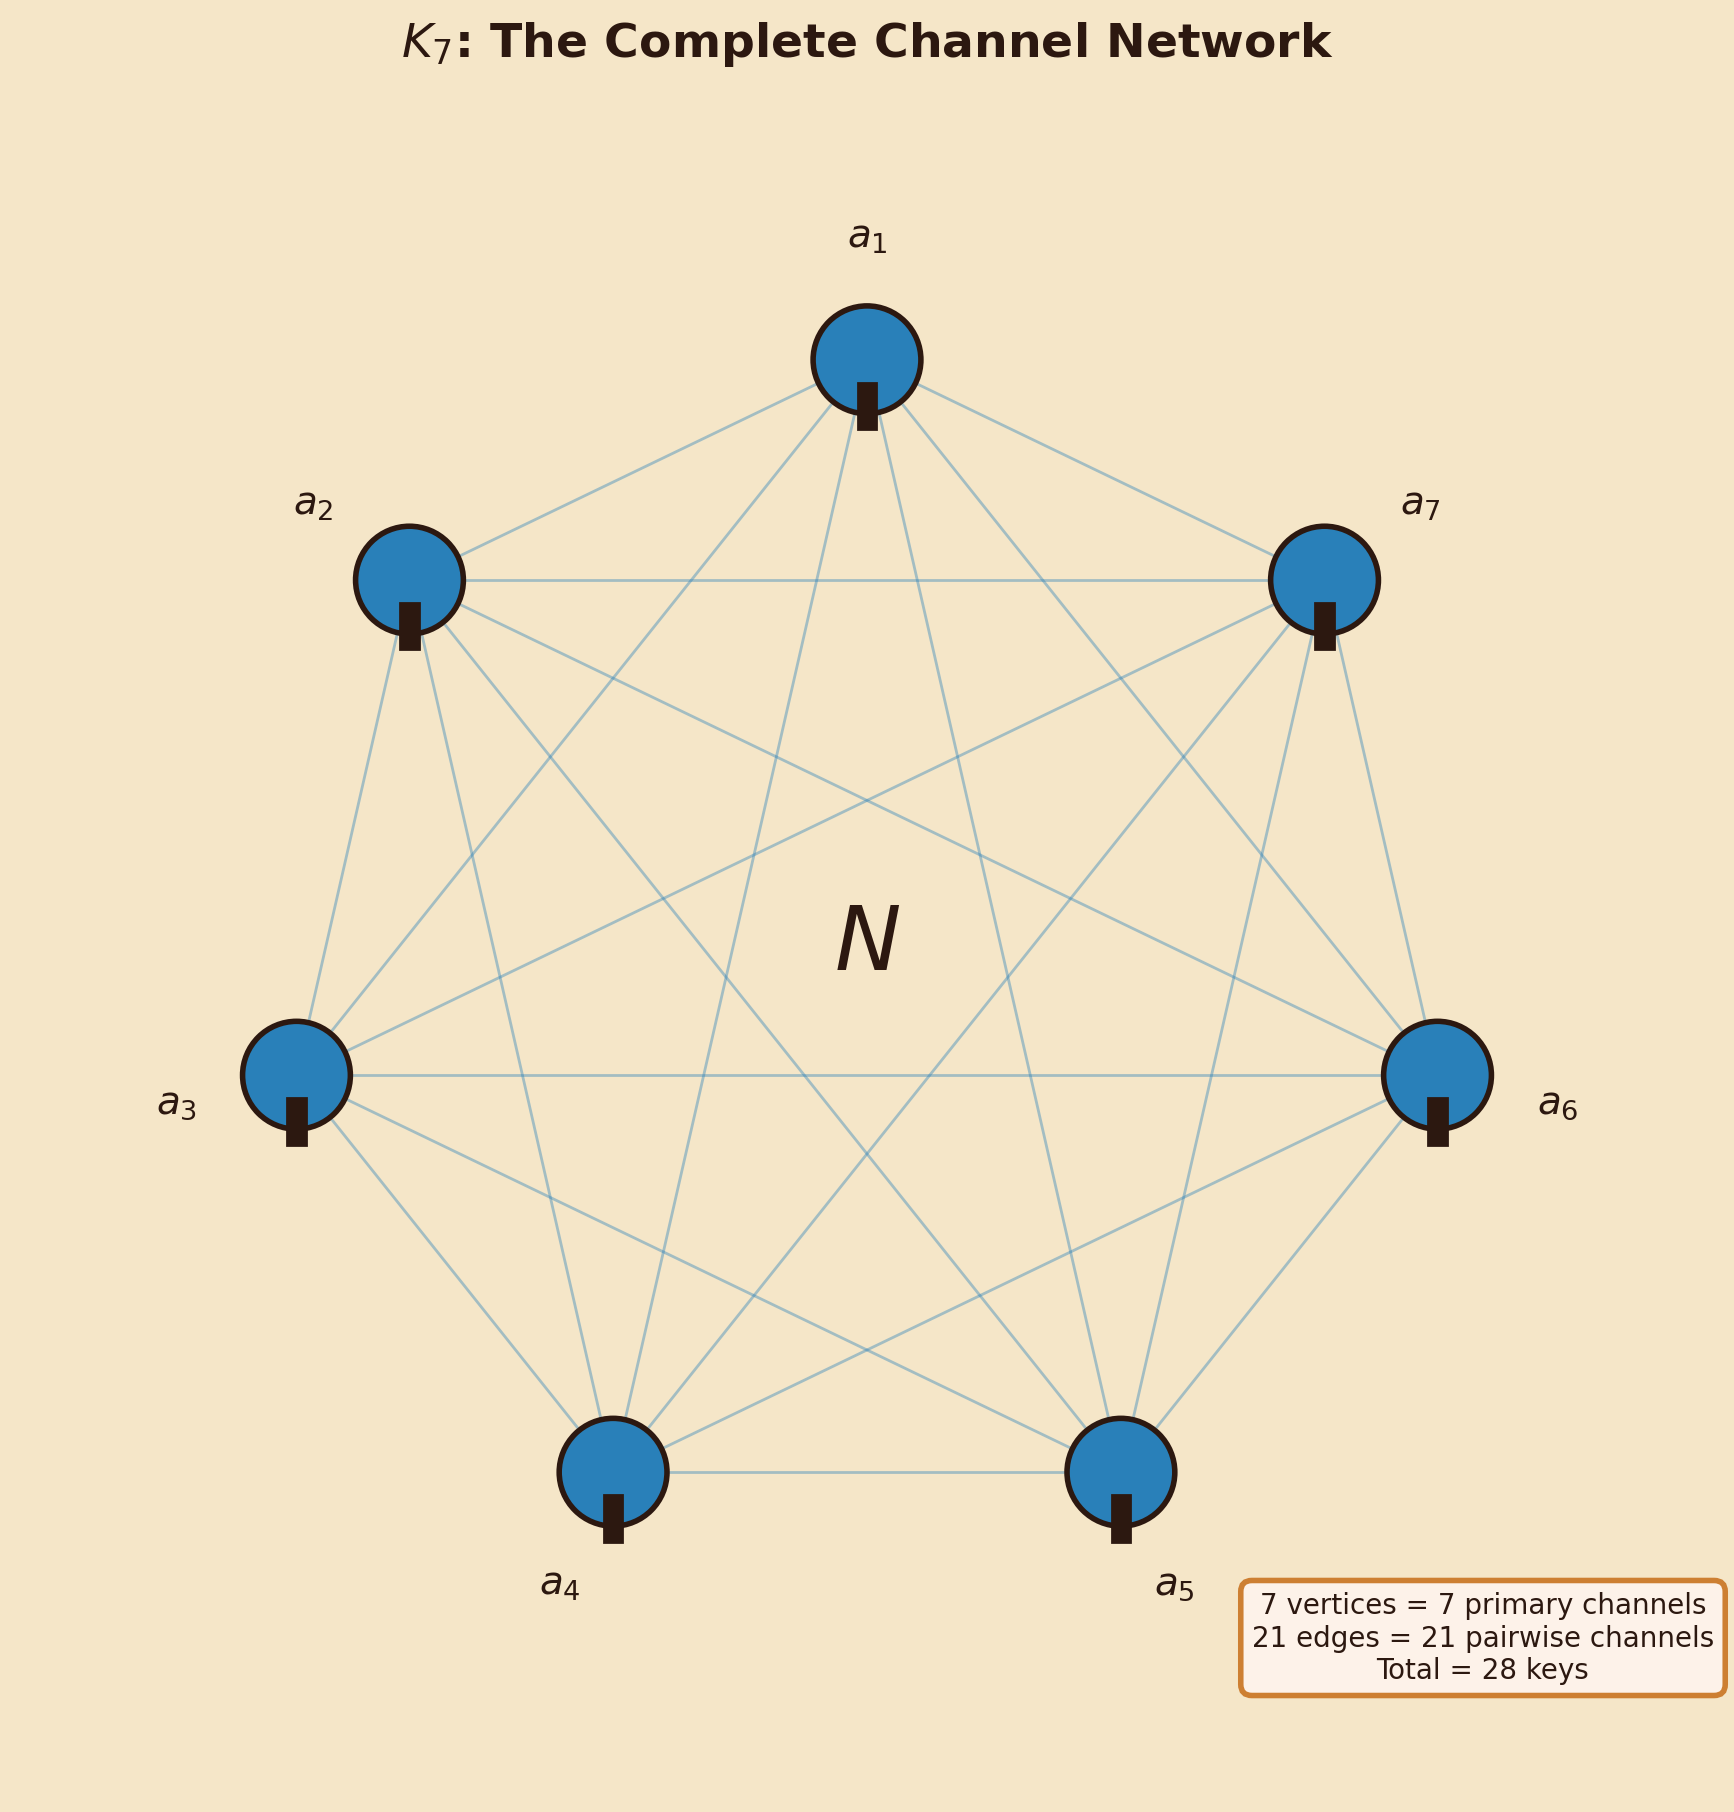
\includegraphics[width=0.82\textwidth]{../Chapter6/images/fig06_K7_channels.png}
\end{figure}


\textbf{A puzzle for the reader.} Given the octuplet \((1, 2, 3, 4, 5, 6, 3, 10)\), compute all seven primary GCDs \(\gcd(10 - a_i, 10)\). Which ones yield nontrivial factors of \(10\)?

The difference-of-squares factorization \(a^2 - b^2 = (a - b)(a + b)\) traces back to Pierre de Fermat, circa 1643. Fermat's method was to search for an integer \(a\) such that \(a^2 - N\) is a perfect square \(b^2\), giving \(N = (a - b)(a + b)\). Our approach inverts this classical strategy: we begin with a multi-term Pythagorean relation and extract \emph{many} difference-of-squares identities simultaneously, like a jeweler cutting multiple facets from a single rough stone.



\section{The Maze Run Backwards --- Inside-Out Factoring}\label{ch6-the-maze-run-backwards-inside-out-factoring}

There is a famous trick for solving mazes: start at the exit and work backwards. The paths that seemed hopeless from the entrance become obvious from the finish. The same trick --- surprisingly powerful, surprisingly underappreciated --- works in factoring.

In all the examples so far, we began with a Pythagorean tuple and checked whether its hypotenuse happened to be the composite number we wished to factor. This is the ``outside-in'' approach: search the vast space of tuples, hope to stumble on one with the right hypotenuse. But what if we turned the maze around?

\textbf{The Inside-Out Parametrization.} Instead of searching for a tuple that \emph{happens} to have hypotenuse \(N\), we \emph{fix} \(N\) as one of the components and ask: what tuples contain it?

In the triple case, given \(N\), we choose any integer \(u\) and check whether

\[h^2 = N^2 + u^2\]

has an integer solution \(h\). If so, we get a Pythagorean triple \((N, u, h)\) and the factoring identity

\[(h - u)(h + u) = N^2,\]

from which \(\gcd(h - u, N)\) may reveal a factor. One free parameter \(u\), one factoring channel.

Now watch what happens when we step up a dimension. In the quadruple case, given \(N\), we choose two integers \(u\) and \(v\) and check whether

\[h^2 = N^2 + u^2 + v^2\]

is a perfect square. If so, we have the quadruple \((N, u, v, h)\) and \emph{two} independent channels:

\[(h - v)(h + v) = N^2 + u^2 \qquad \text{and} \qquad (h - u)(h + u) = N^2 + v^2.\]

Two free parameters, two factoring channels. You see the pattern emerging.

\begin{quote}
\textbf{The Dimension Advantage Theorem.} In dimension \(k\), the inside-out method has \(k - 2\) free parameters \(u_1, \ldots, u_{k-2}\). Each parameter provides an independent factoring channel. More dimensions, more freedom, more chances.
\end{quote}

The metaphor is irresistible. In three dimensions, you are a mole tunneling through rock, with one degree of freedom for your tunnel direction. In four dimensions, you are a bird that can also choose altitude. In five dimensions, you are something for which English has no name --- but you have three independent directions to explore. And in eight dimensions, you are an octopus with seven tentacles, each probing a different direction simultaneously.


\begin{figure}[htbp]
\centering
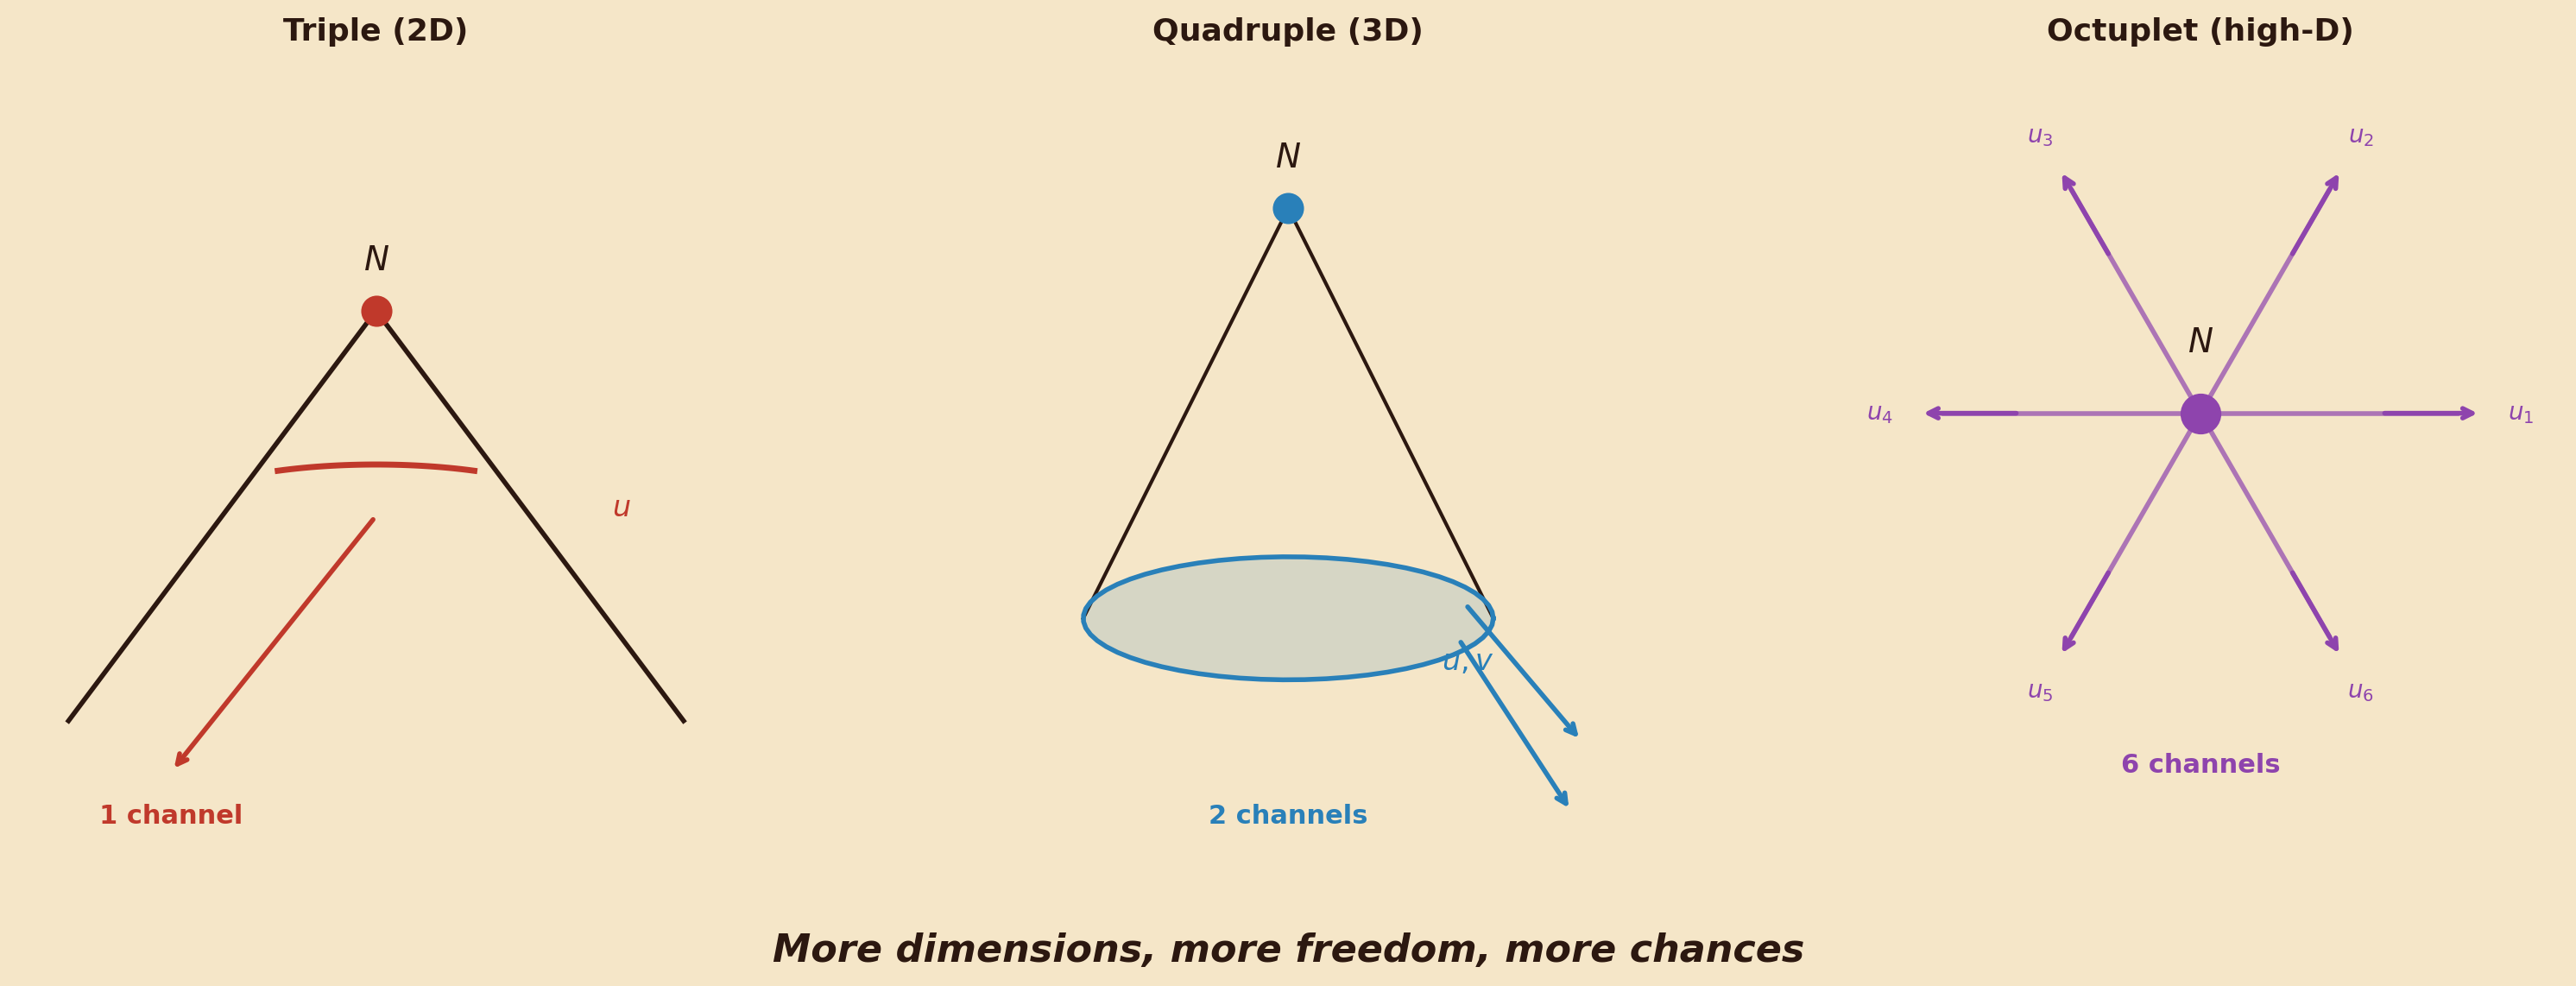
\includegraphics[width=0.82\textwidth]{../Chapter6/images/fig07_inside_out.png}
\end{figure}



\begin{figure}[htbp]
\centering
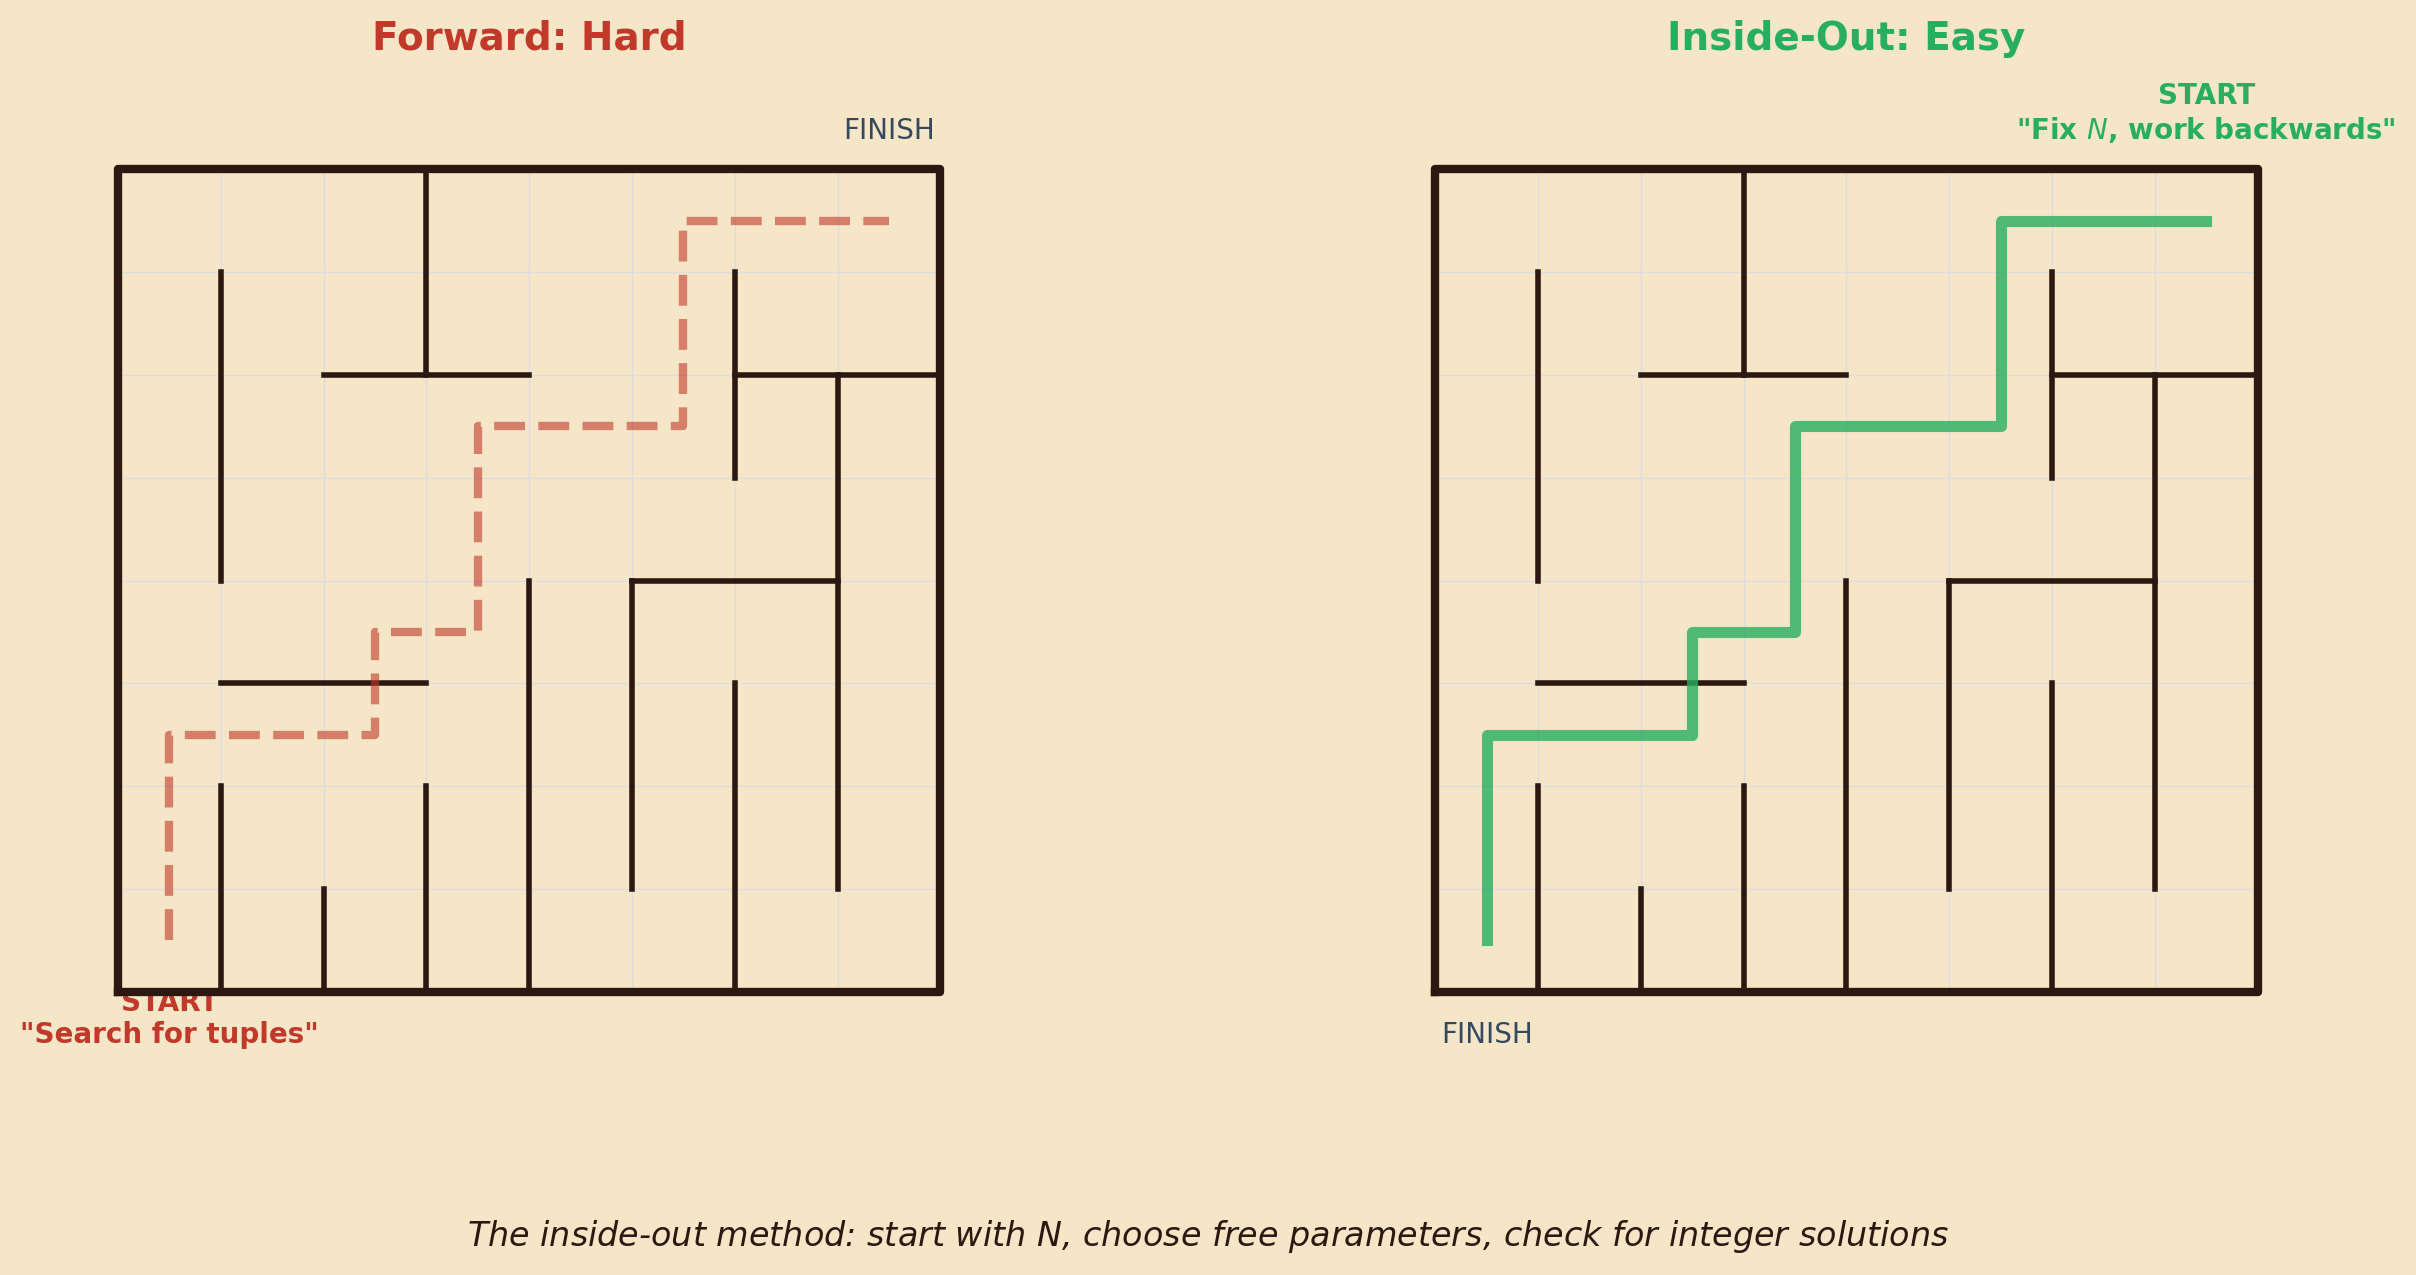
\includegraphics[width=0.82\textwidth]{../Chapter6/images/fig08_maze.png}
\end{figure}




\section{Sisyphus and the Number Theorist --- Climbing and Falling}\label{ch6-sisyphus-and-the-number-theorist-climbing-and-falling}

In Greek myth, Sisyphus was condemned to roll a boulder up a hill, only to watch it roll back down for eternity. In the Pythagorean world, the situation is more fortunate --- but the metaphor holds: going \emph{up} the tree (building ever-larger tuples) is easy; going \emph{down} the tree (reducing the hypotenuse to find its hidden structure) is hard. But the beautiful thing is that \emph{down} is where the factors hide.

In Chapter 1, we met the \index{Berggren tree}Berggren tree and its three generating matrices. We learned that every primitive Pythagorean triple can be reached from the seed \((3, 4, 5)\) by applying sequences of the matrices \(\mathbf{A}\), \(\mathbf{B}\), \(\mathbf{C}\). That is the ascent --- the enumeration phase. Now let us study the descent.

\textbf{The Inverse Berggren Transform.} Consider one of the three inverses, which we will call \(B_2^{-1}\). It acts on a triple \((a, b, c)\) by the rule:

\[B_2^{-1}(a, b, c) = \big(a + 2b - 2c,\;\; 2a + b - 2c,\;\; -2a - 2b + 3c\big).\]

Let us call the output \((a', b', c')\). The first wonderful fact is that this map preserves the Pythagorean property: if \(a^2 + b^2 = c^2\), then \(a'^2 + b'^2 = c'^2\). The parent is again a Pythagorean triple. You can verify this by a (somewhat tedious but wholly elementary) expansion of both sides.

The second wonderful fact is the \textbf{Hypotenuse Descent Theorem}: the parent's hypotenuse is strictly smaller than the child's:

\[c' = -2a - 2b + 3c < c.\]

Why? Because \((a + b - c)^2 \geq 0\) --- the square of any real number is nonnegative --- which expands to \(a^2 + b^2 + c^2 + 2ab - 2ac - 2bc \geq 0\). Using \(a^2 + b^2 = c^2\), this simplifies to \(2c^2 + 2ab - 2ac - 2bc \geq 0\), hence \(c^2 \geq c(a + b) - ab \geq c(a + b - c)\). A bit more algebra gives \(3c - 2a - 2b \leq c\), with equality only in degenerate cases.

The third fact: the parent hypotenuse remains \emph{positive}. We have \(c' = 3c - 2a - 2b > 0\), which follows from the sharper inequality \(c < a + b\) (the triangle inequality --- the hypotenuse is always shorter than the sum of the two legs).

So the descent is genuine: each step shrinks the hypotenuse, the hypotenuse stays positive, and the Pythagorean property is preserved. Eventually, every primitive triple must descend to the root \((3, 4, 5)\). The tree has a single taproot.

The duality is now clear:

\begin{itemize}

\item
  \textbf{Ascent} (up the tree) \(=\) \emph{enumeration}: generating all \(k\)-tuples with bounded hypotenuse.
\item
  \textbf{Descent} (down the tree) \(=\) \emph{factoring}: reducing the hypotenuse to reveal algebraic structure.
\end{itemize}

Going up is easy --- just multiply by a matrix. Going down is hard --- you must choose the right inverse at each step. But the factors of \(N\) are buried in the descent path, like fossils in layers of rock.


\begin{figure}[htbp]
\centering
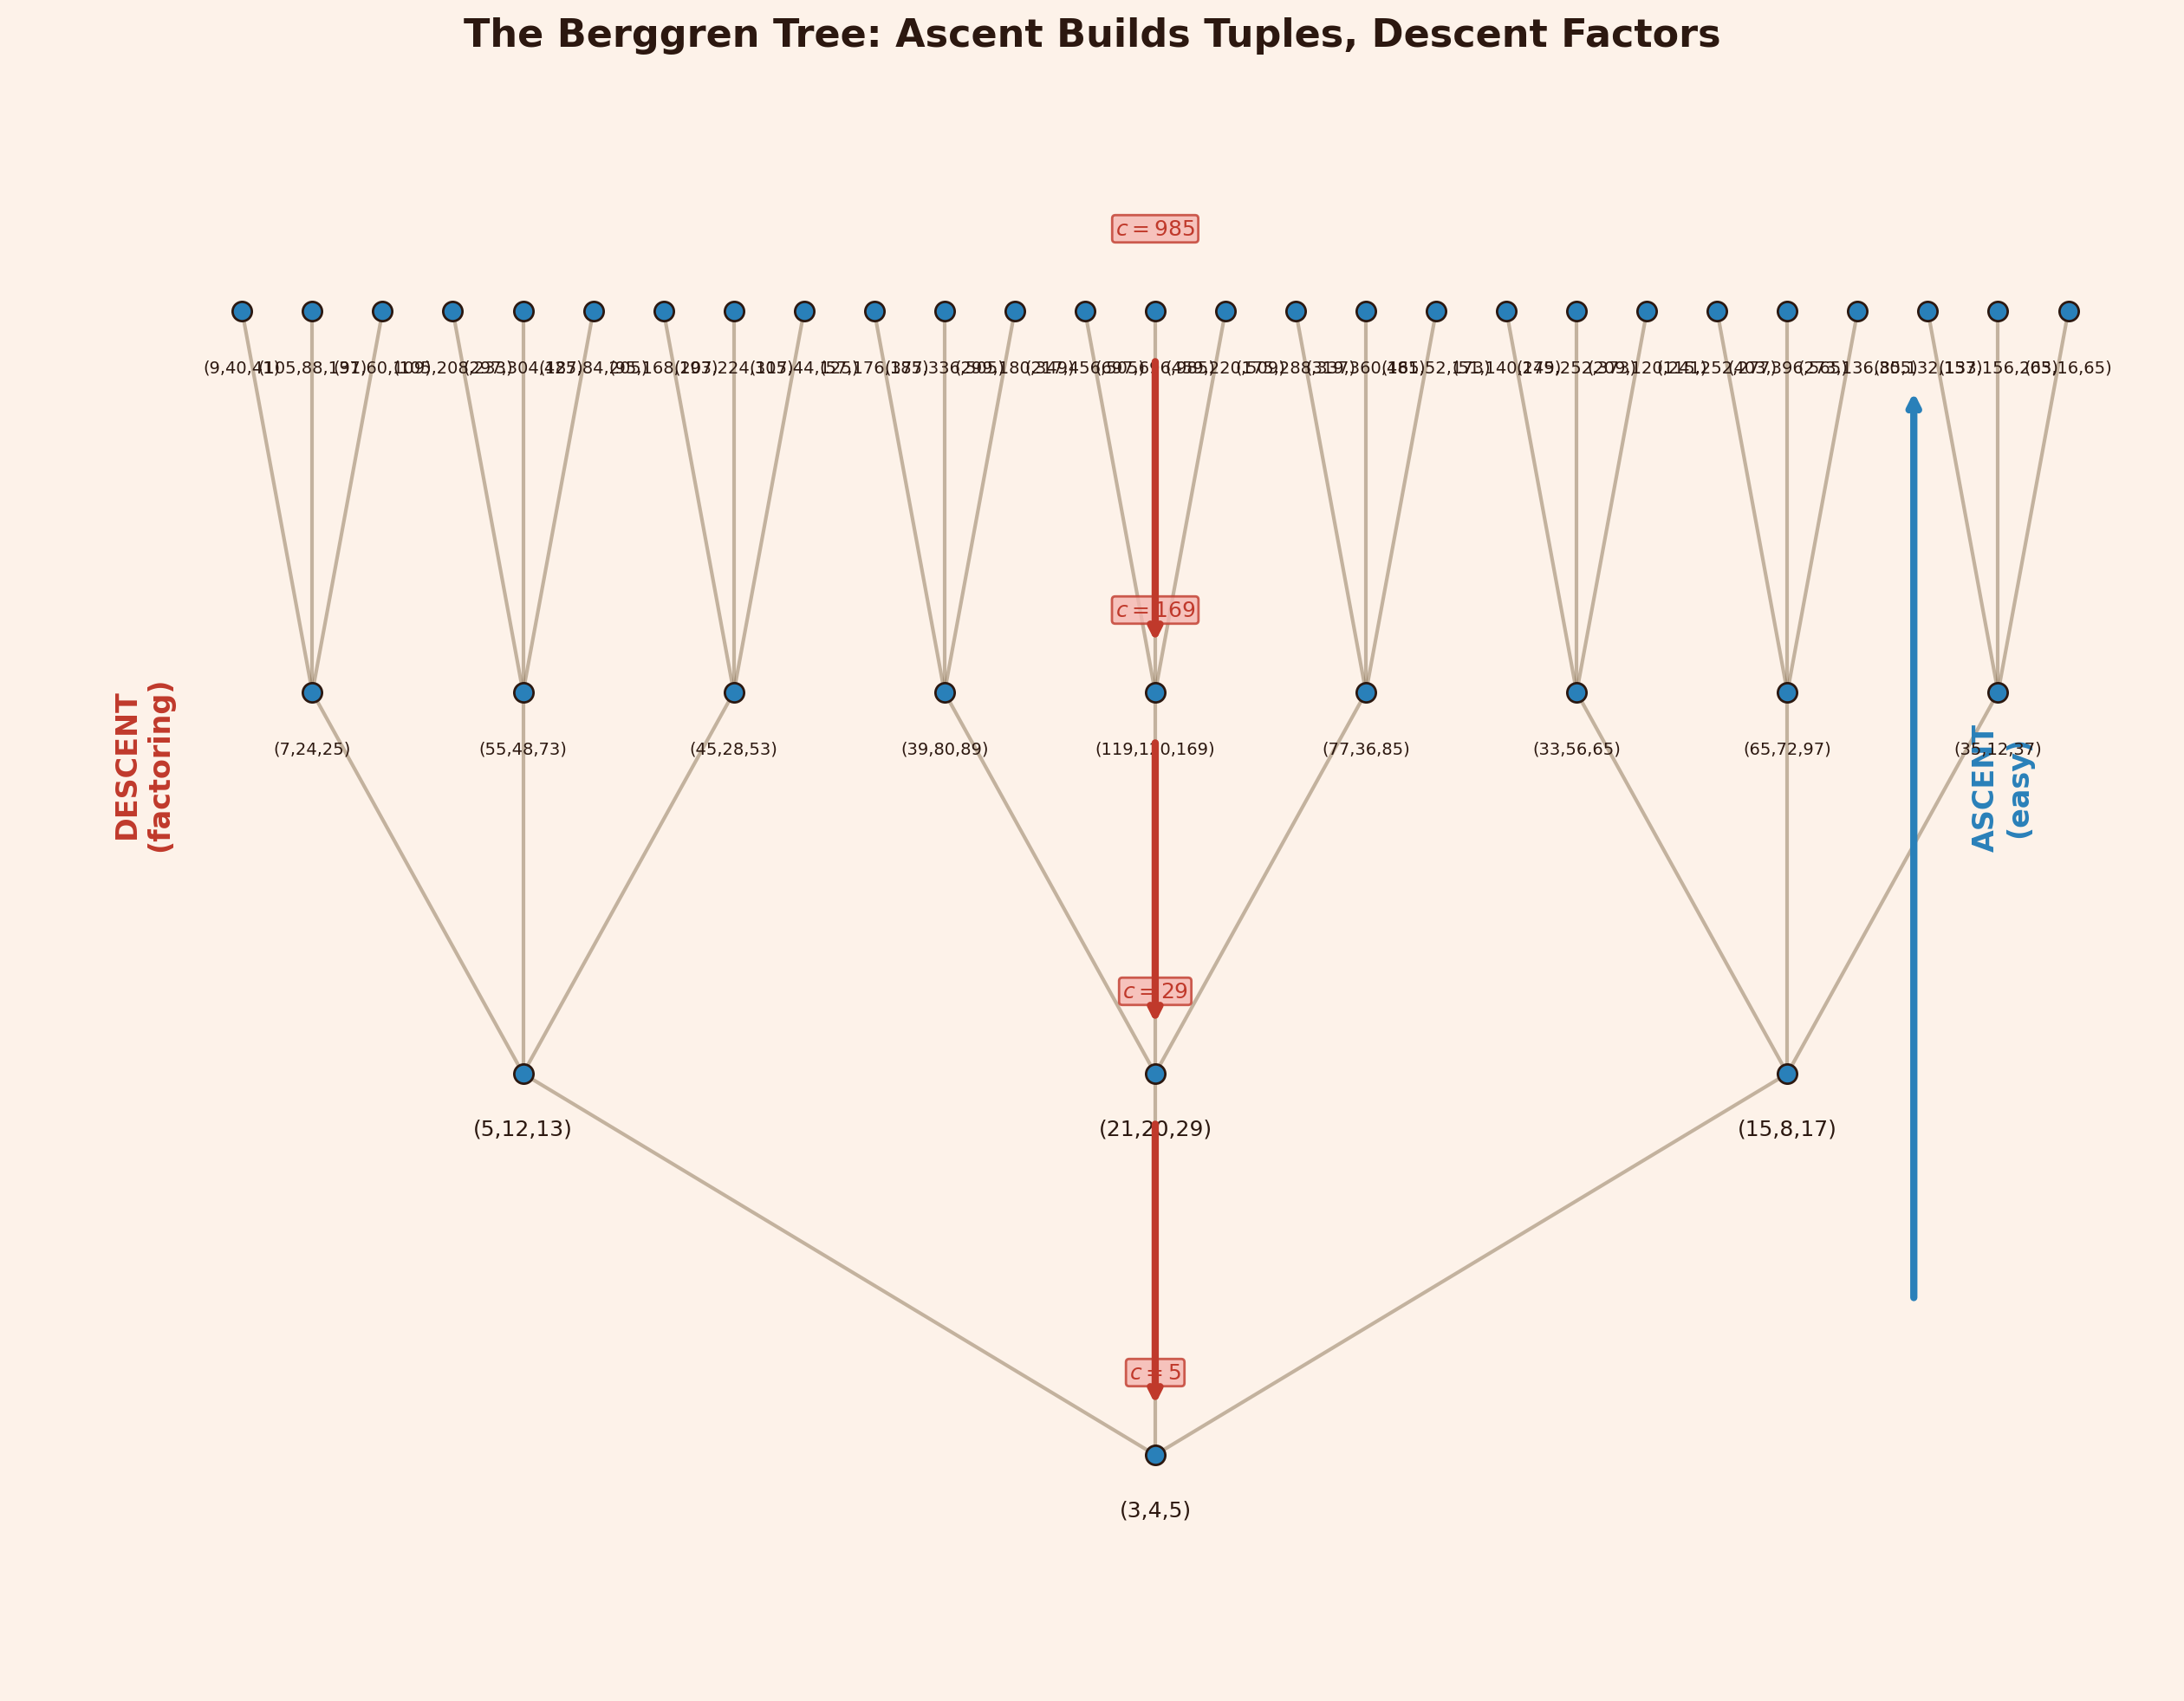
\includegraphics[width=0.82\textwidth]{../Chapter6/images/fig09_berggren_descent.png}
\end{figure}




\section{\texorpdfstring{The Hall of Mirrors --- The Reflection \(R_{1111}\) and the Quadruple Forest}{The Hall of Mirrors --- The Reflection R\_\{1111\} and the Quadruple Forest}}\label{ch6-the-hall-of-mirrors-the-reflection-r_1111-and-the-quadruple-forest}

Step into a hall of mirrors, and your reflection tells you something about yourself that you can't see directly --- a reversed image, but one that is undeniably \emph{you}. In the world of Pythagorean quadruples, there is a remarkable ``reflection'' --- a map that sends one quadruple to another while preserving the sum-of-squares equation. And the reflected image reveals factors of the original hypotenuse.

\textbf{The \(R_{1111}\) Reflection.} Given a Pythagorean quadruple \((a, b, c, d)\) with \(a^2 + b^2 + c^2 = d^2\), define:

\[R_{1111}(a, b, c, d) = \big(d - b - c,\;\; d - a - c,\;\; d - a - b,\;\; 2d - a - b - c\big).\]

This looks like a strange recipe --- subtract pairs of components from the hypotenuse, and form a new hypotenuse from the old one minus all three. But watch what happens. The \textbf{Preservation Theorem} states: if \(a^2 + b^2 + c^2 = d^2\), then the reflected quadruple satisfies the same equation:

\[(d - b - c)^2 + (d - a - c)^2 + (d - a - b)^2 = (2d - a - b - c)^2.\]

You can verify this by expanding both sides and using \(a^2 + b^2 + c^2 = d^2\) to simplify. The algebra is a satisfying exercise --- not deep, but surprisingly clean.

The \textbf{Descent Factor Channel} is where the magic happens. When \(d = N\) is our target composite, the reflected spatial components \(N - b - c\), \(N - a - c\), \(N - a - b\) are linear combinations of \(N\) and the original components. Each one provides a factoring channel:

\[\gcd(N - b - c, \, N), \qquad \gcd(N - a - c, \, N), \qquad \gcd(N - a - b, \, N).\]

All three divide \(N\). If any of them is nontrivial --- strictly between \(1\) and \(N\) --- we've factored \(N\).

And the reflection genuinely \emph{descends}. The \textbf{Descent Energy Theorem} states: when \(a, b, c > 0\), the reflected hypotenuse satisfies

\[2d - a - b - c < d.\]

The proof is a one-liner: \(d^2 = a^2 + b^2 + c^2 < (a + b + c)^2\) (because the cross terms \(2ab + 2ac + 2bc\) are all positive), so \(d < a + b + c\), and therefore \(2d - a - b - c < d\). The mirror \emph{shrinks} the hypotenuse. Each reflection brings us closer to the base cases --- closer to the factors.


\begin{figure}[htbp]
\centering
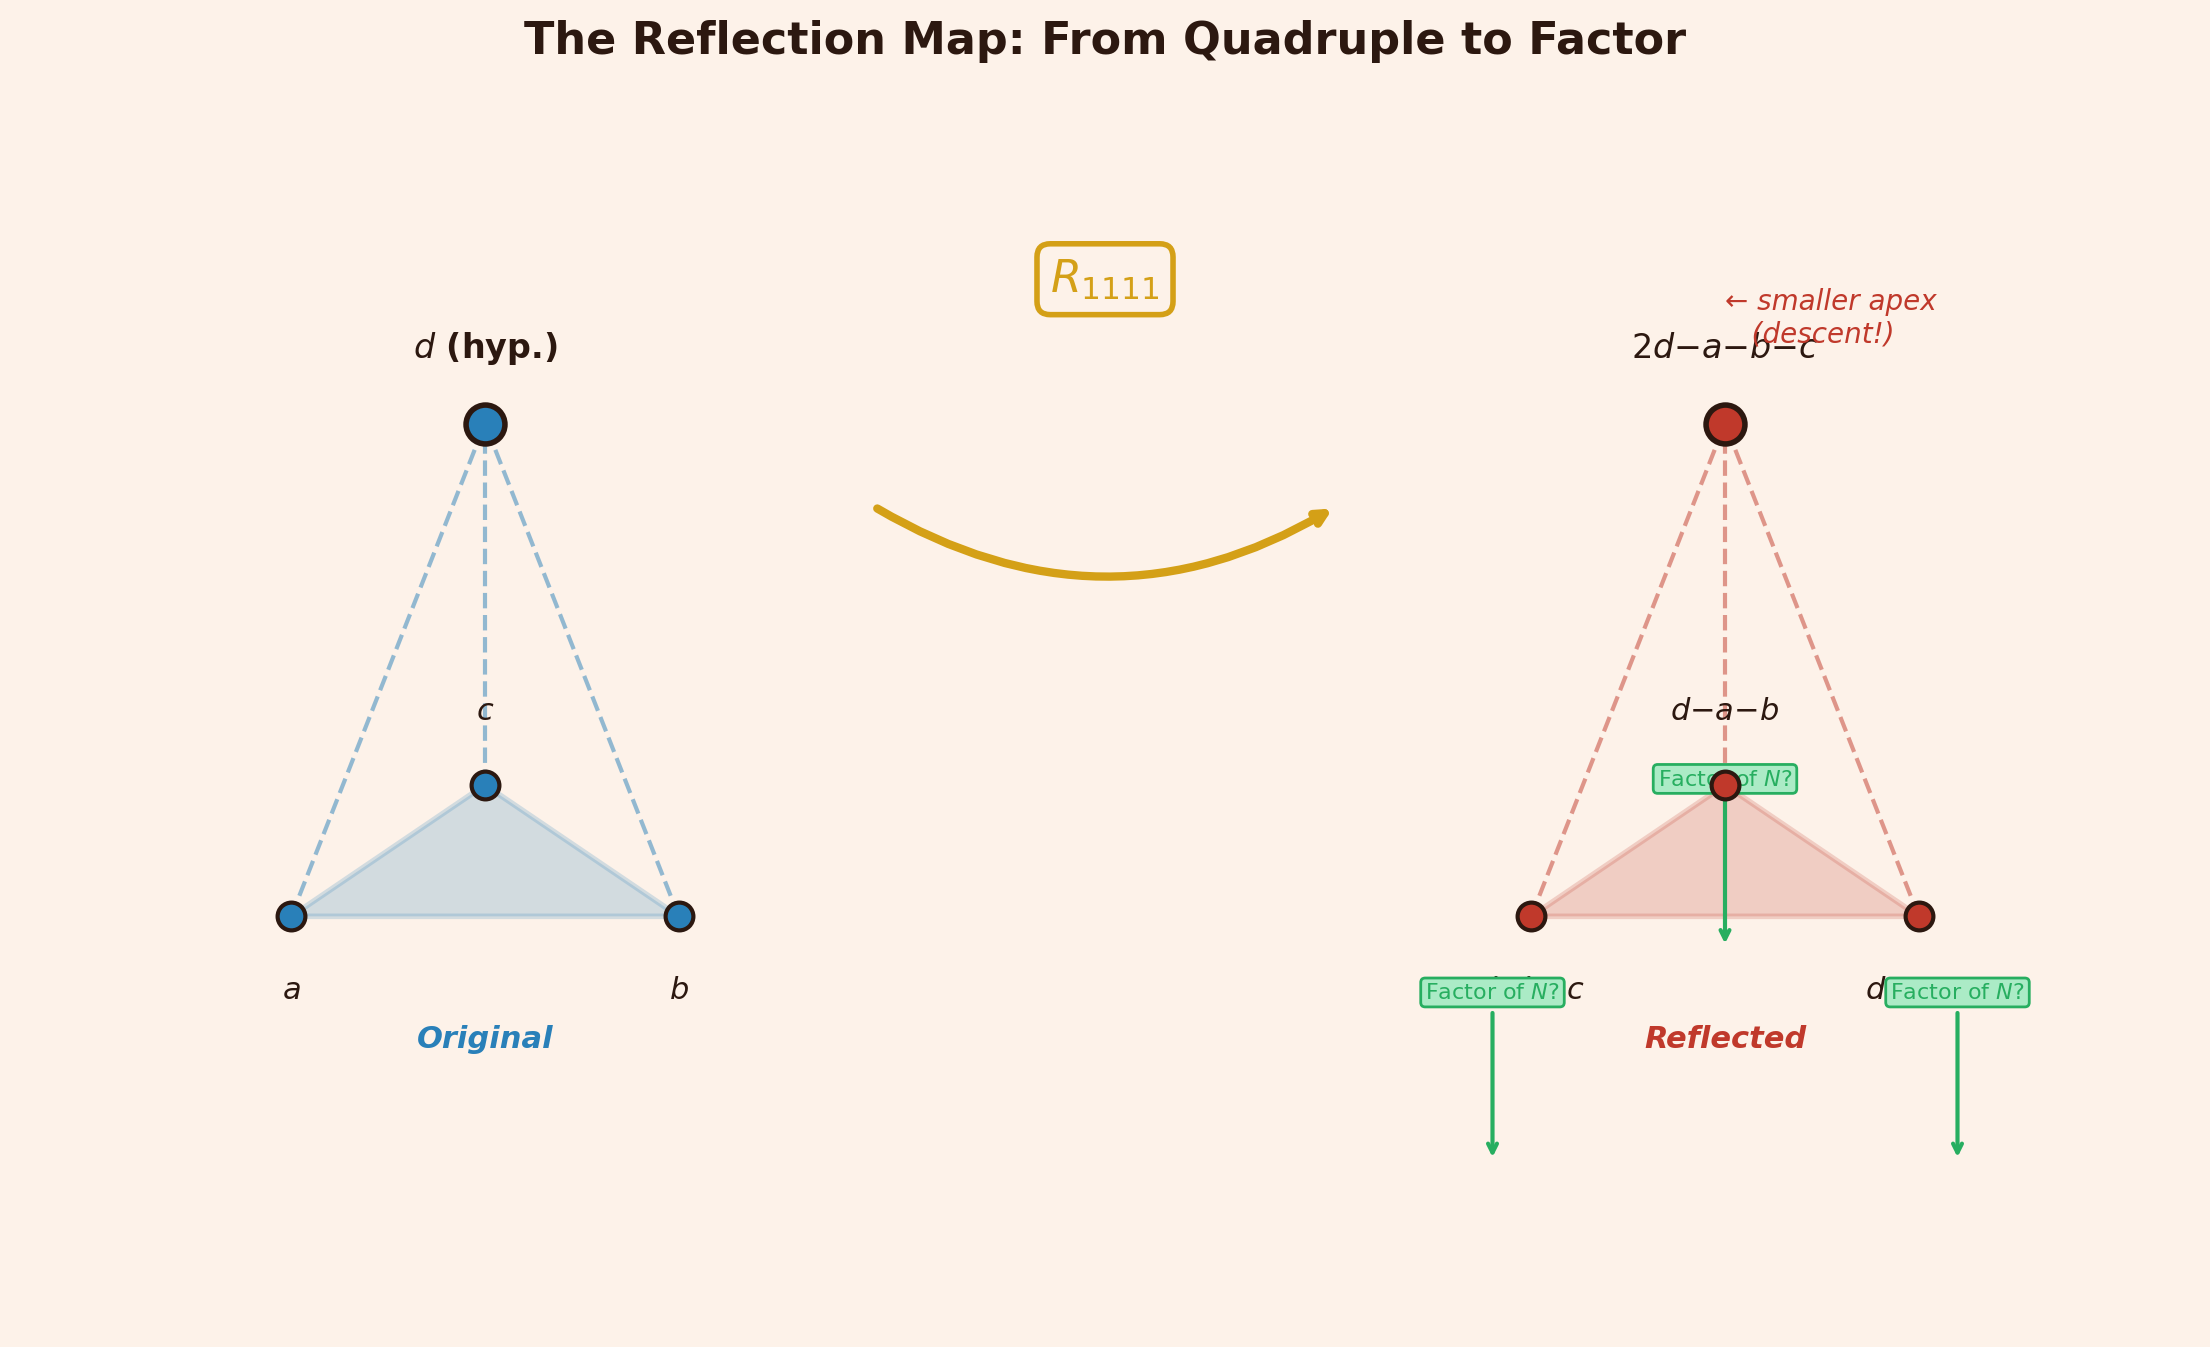
\includegraphics[width=0.82\textwidth]{../Chapter6/images/fig10_reflection_tetrahedra.png}
\end{figure}


\textbf{A puzzle for the reader.} Apply \(R_{1111}\) to the quadruple \((5, 10, 10, 15)\). Verify that the result is again a valid Pythagorean quadruple. What is the reflected hypotenuse? What factoring channels does the reflected quadruple provide for \(N = 15\)?



\section{The Elevator Between Floors --- Lifting, Projection, and Chain Composition}\label{ch6-the-elevator-between-floors-lifting-projection-and-chain-composition}

Imagine a building where each floor represents a different dimension of Pythagorean tuples: Floor 3 is triples, Floor 4 is quadruples, Floor 5 is quintuplets, and so on up to Floor 8. There are elevators connecting them --- and the remarkable thing is that they go \emph{both ways}. You can ride up (lifting) or down (projection), and the factoring information survives the trip.

\textbf{Trivial Lifting.} Any Pythagorean triple \((a, b, c)\) with \(a^2 + b^2 = c^2\) trivially lifts to a quadruple by inserting a zero:

\[a^2 + b^2 + 0^2 = c^2.\]

And to a quintuplet: \(a^2 + b^2 + 0^2 + 0^2 = c^2\). The zeros are freeloaders --- they contribute nothing to the sum of squares, but they increase the dimension and therefore the number of channels. (The zero-channels, \(\gcd(N - 0, N) = N\), are useless, of course. The free ride has its limits.)

\textbf{Nontrivial Lifting via Chain Composition.} Here is a far more interesting elevator. Suppose we have two Pythagorean triples that share a component:

\[a^2 + b^2 = c^2 \qquad \text{and} \qquad c^2 + d^2 = e^2.\]

The first triple's hypotenuse \(c\) is a leg of the second triple. Substituting:

\[a^2 + b^2 + d^2 = c^2 + d^2 = e^2.\]

The intermediate value \(c\) cancels, and we have lifted two triples into a single quadruple \((a, b, d, e)\). The nontrivial lift has created a \emph{new} factoring channel (via \(d\)) that existed in neither parent triple alone.

For example: \((3, 4, 5)\) and \((5, 12, 13)\) chain to give \((3, 4, 12, 13)\):

\[3^2 + 4^2 + 12^2 = 9 + 16 + 144 = 169 = 13^2. \checkmark\]

The lift adds the channel \(\gcd(13 - 12, 13) = \gcd(1, 13) = 1\) --- not helpful in this case. But the principle is powerful: chain composition lets us systematically build higher-dimensional tuples from lower-dimensional ones, each lift potentially adding useful channels.

\textbf{Cross-Dimensional Projection --- Peeling.} Going downward: from a quintuplet \(a^2 + b^2 + c^2 + d^2 = N^2\), ``peel off'' one component:

\[a^2 + b^2 + c^2 = N^2 - d^2 = (N - d)(N + d).\]

This reduces a five-dimensional factoring problem to a four-dimensional one, but with a \emph{product} on the right instead of a square. Each peeling reveals different algebraic structure.

\textbf{The Channel Cascade.} From a quintuplet with hypotenuse \(N\) and four spatial components, three independent peeling equations emerge:

\[\begin{aligned}
(N - d)(N + d) &= a^2 + b^2 + c^2 \\
(N - c)(N + c) &= a^2 + b^2 + d^2 \\
(N - b)(N + b) &= a^2 + c^2 + d^2
\end{aligned}\]

Each equation offers a different window into the factorization of \(N\). The elevator rides up and down, and at every floor, there is something new to see.


\begin{figure}[htbp]
\centering
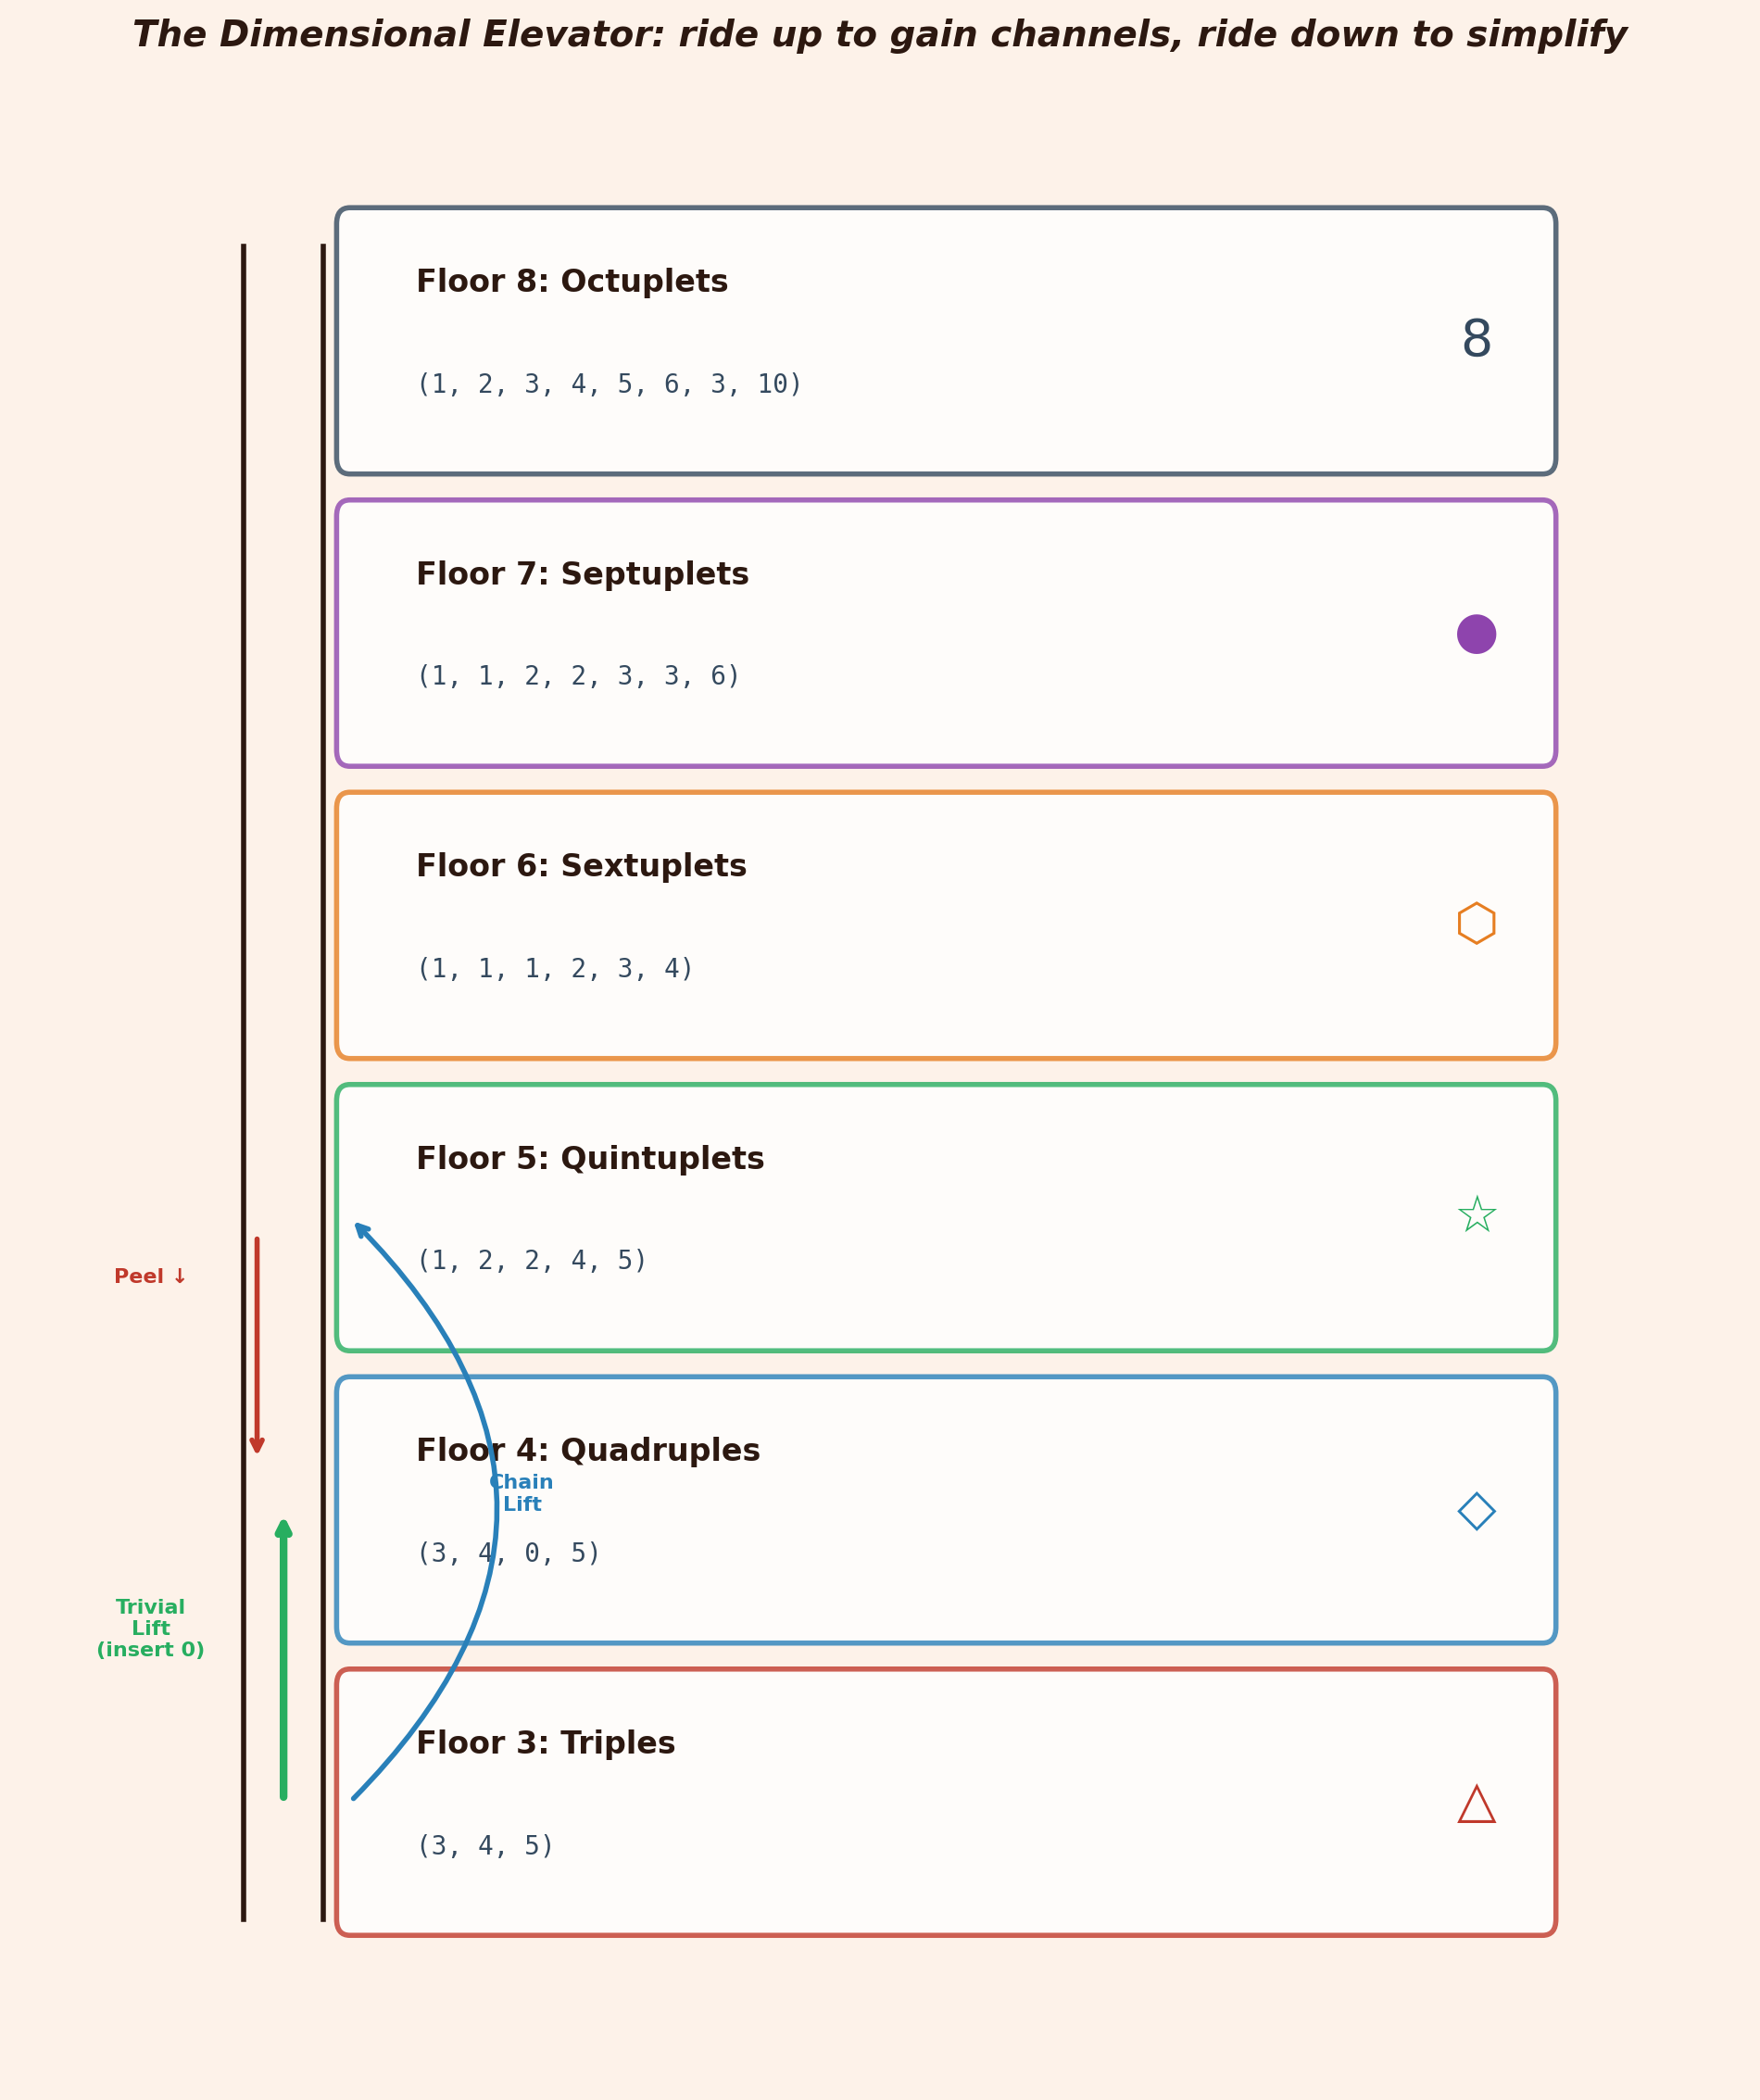
\includegraphics[width=0.82\textwidth]{../Chapter6/images/fig11_dimensional_elevator.png}
\end{figure}




\section{The Magic Trick That's 1,400 Years Old --- Brahmagupta, Fibonacci, and Euler}\label{ch6-the-magic-trick-thats-1400-years-old-brahmagupta-fibonacci-and-euler}

In 628 AD, the Indian mathematician Brahmagupta discovered something astonishing: the product of two numbers, each of which is a sum of two squares, is \emph{always itself} a sum of two squares. A thousand years later, Euler found the four-square version. These ancient identities are not merely beautiful --- they are \emph{multiplication theorems for factoring channels}.

\textbf{The Brahmagupta--Fibonacci Identity.} For any four integers \(a, b, c, d\):

\[(a^2 + b^2)(c^2 + d^2) = (ac - bd)^2 + (ad + bc)^2.\]

Check it: expand both sides, and everything cancels except the desired sum of two squares on the right. The identity says: if \(N_1 = a^2 + b^2\) and \(N_2 = c^2 + d^2\), then \(N_1 \cdot N_2\) is also a sum of two squares, and we know \emph{explicitly} which two squares they are. The product inherits the structure of its factors.

\textbf{The Euler Four-Square Identity.} For any eight integers \(a_1, a_2, a_3, a_4\) and \(b_1, b_2, b_3, b_4\):

\[(a_1^2 + a_2^2 + a_3^2 + a_4^2)(b_1^2 + b_2^2 + b_3^2 + b_4^2) = c_1^2 + c_2^2 + c_3^2 + c_4^2,\]

where

\[\begin{aligned}
c_1 &= a_1 b_1 - a_2 b_2 - a_3 b_3 - a_4 b_4, \\
c_2 &= a_1 b_2 + a_2 b_1 + a_3 b_4 - a_4 b_3, \\
c_3 &= a_1 b_3 - a_2 b_4 + a_3 b_1 + a_4 b_2, \\
c_4 &= a_1 b_4 + a_2 b_3 - a_3 b_2 + a_4 b_1.
\end{aligned}\]

Those sixteen terms look formidable --- but they are nothing other than the multiplication rule for \emph{quaternions}, the four-dimensional number system discovered by Hamilton in 1843 (in a flash of inspiration on Brougham Bridge in Dublin, which he celebrated by carving the defining equation \(i^2 = j^2 = k^2 = ijk = -1\) into the stone). The Euler four-square identity is secretly the statement that \index{quaternions}quaternion multiplication preserves norms: \(|pq| = |p| \cdot |q|\) for quaternions \(p, q \in \mathbb{H}\).

\textbf{The Channel Composition Theorem.} These identities let us \emph{compose} factoring channels. If \(a^2 + b^2 = N_1\) and \(c^2 + d^2 = N_2\), then

\[(ac - bd)^2 + (ad + bc)^2 = N_1 \cdot N_2.\]

We have combined two separate Pythagorean representations into a representation of their product. If \(N_1\) and \(N_2\) are both factors of some larger number \(M\), the composed identity gives a Pythagorean representation of \(M\) --- one with potentially more useful channels than either parent had alone.


\begin{figure}[htbp]
\centering
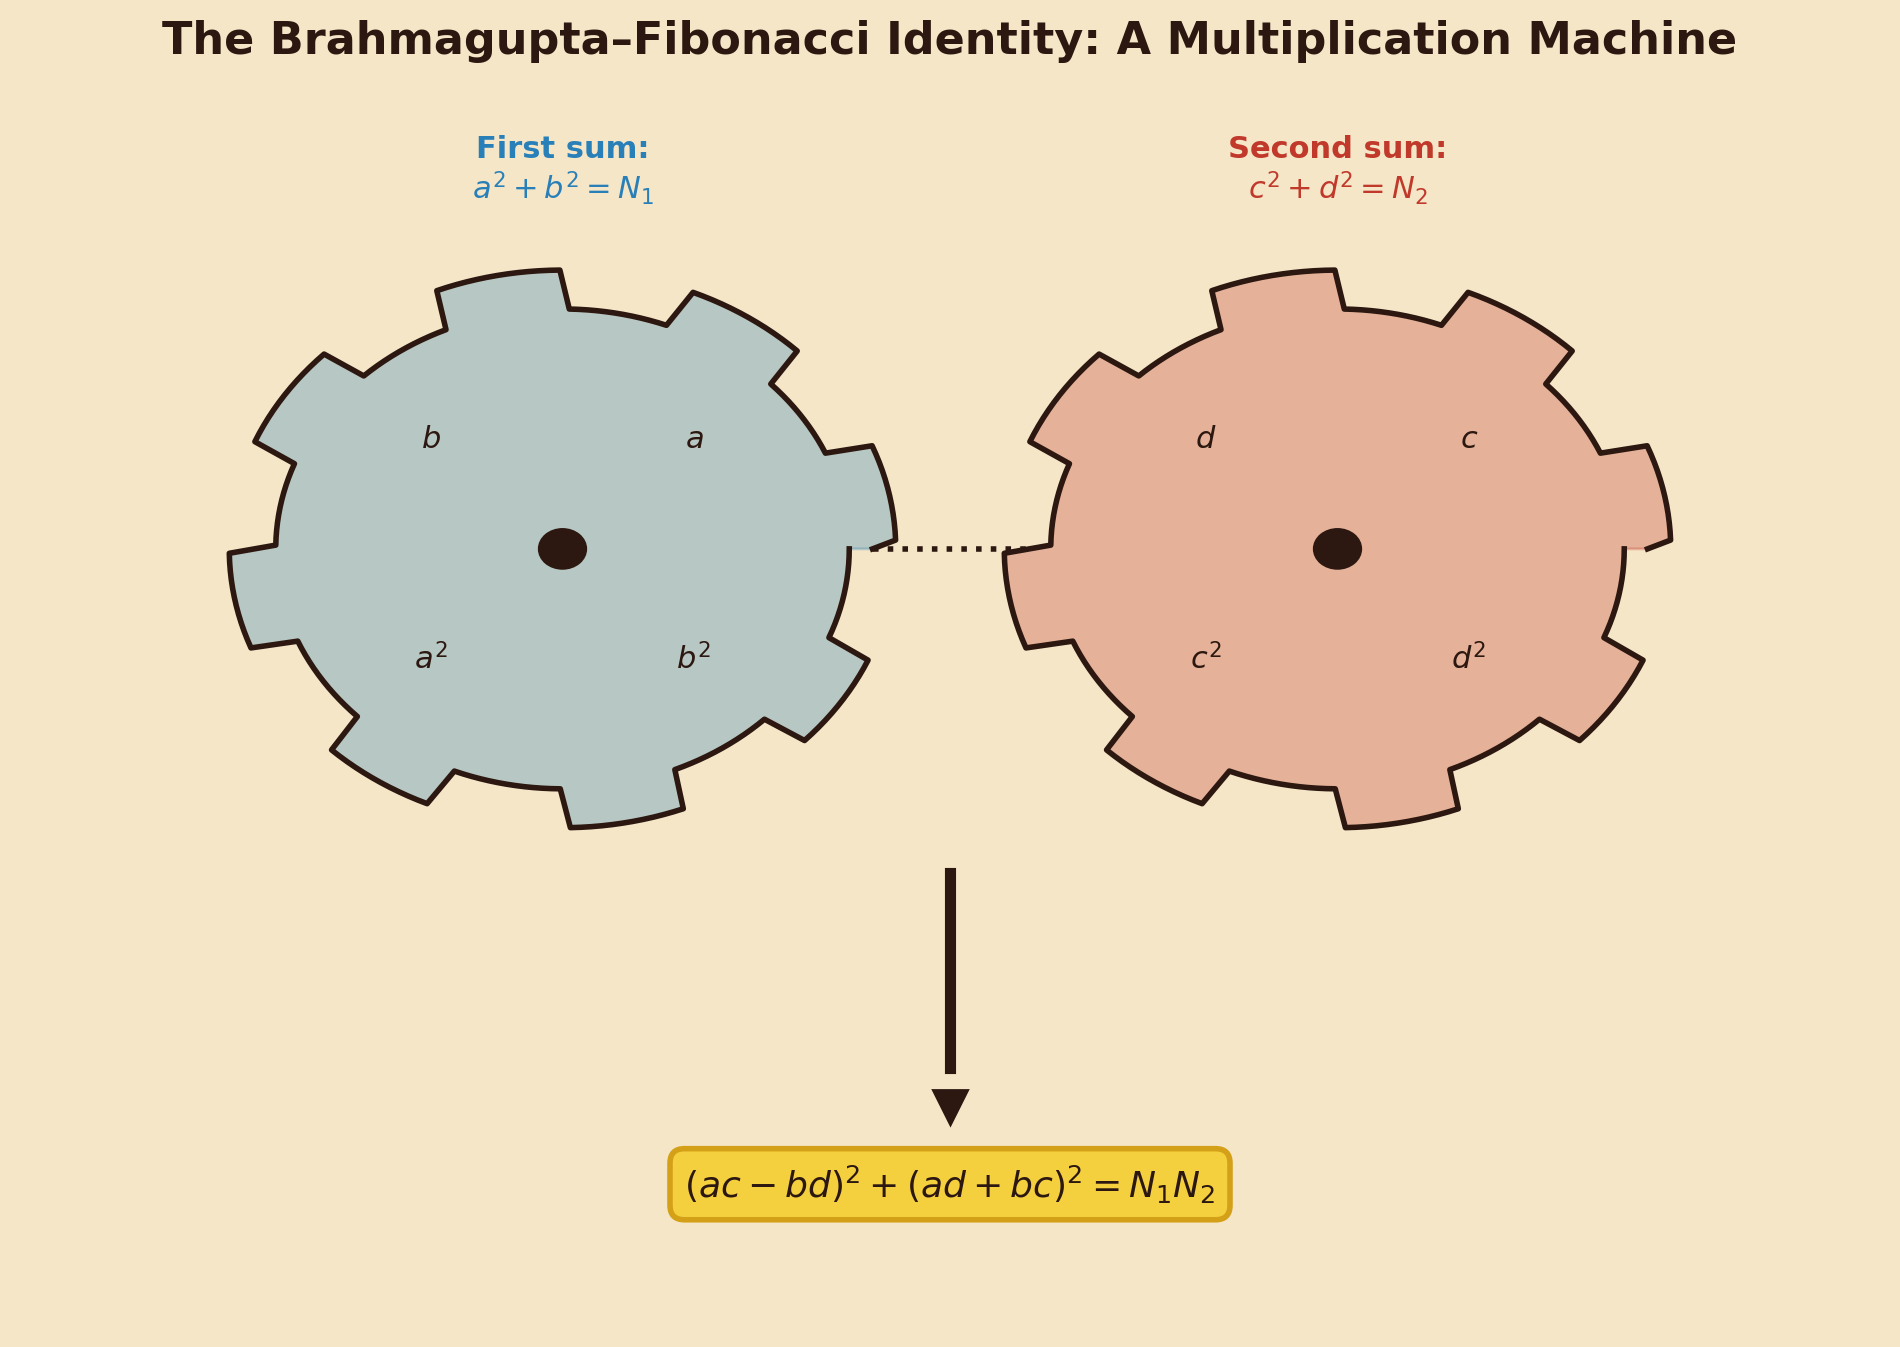
\includegraphics[width=0.82\textwidth]{../Chapter6/images/fig12_gear_machine.png}
\end{figure}



\begin{figure}[htbp]
\centering
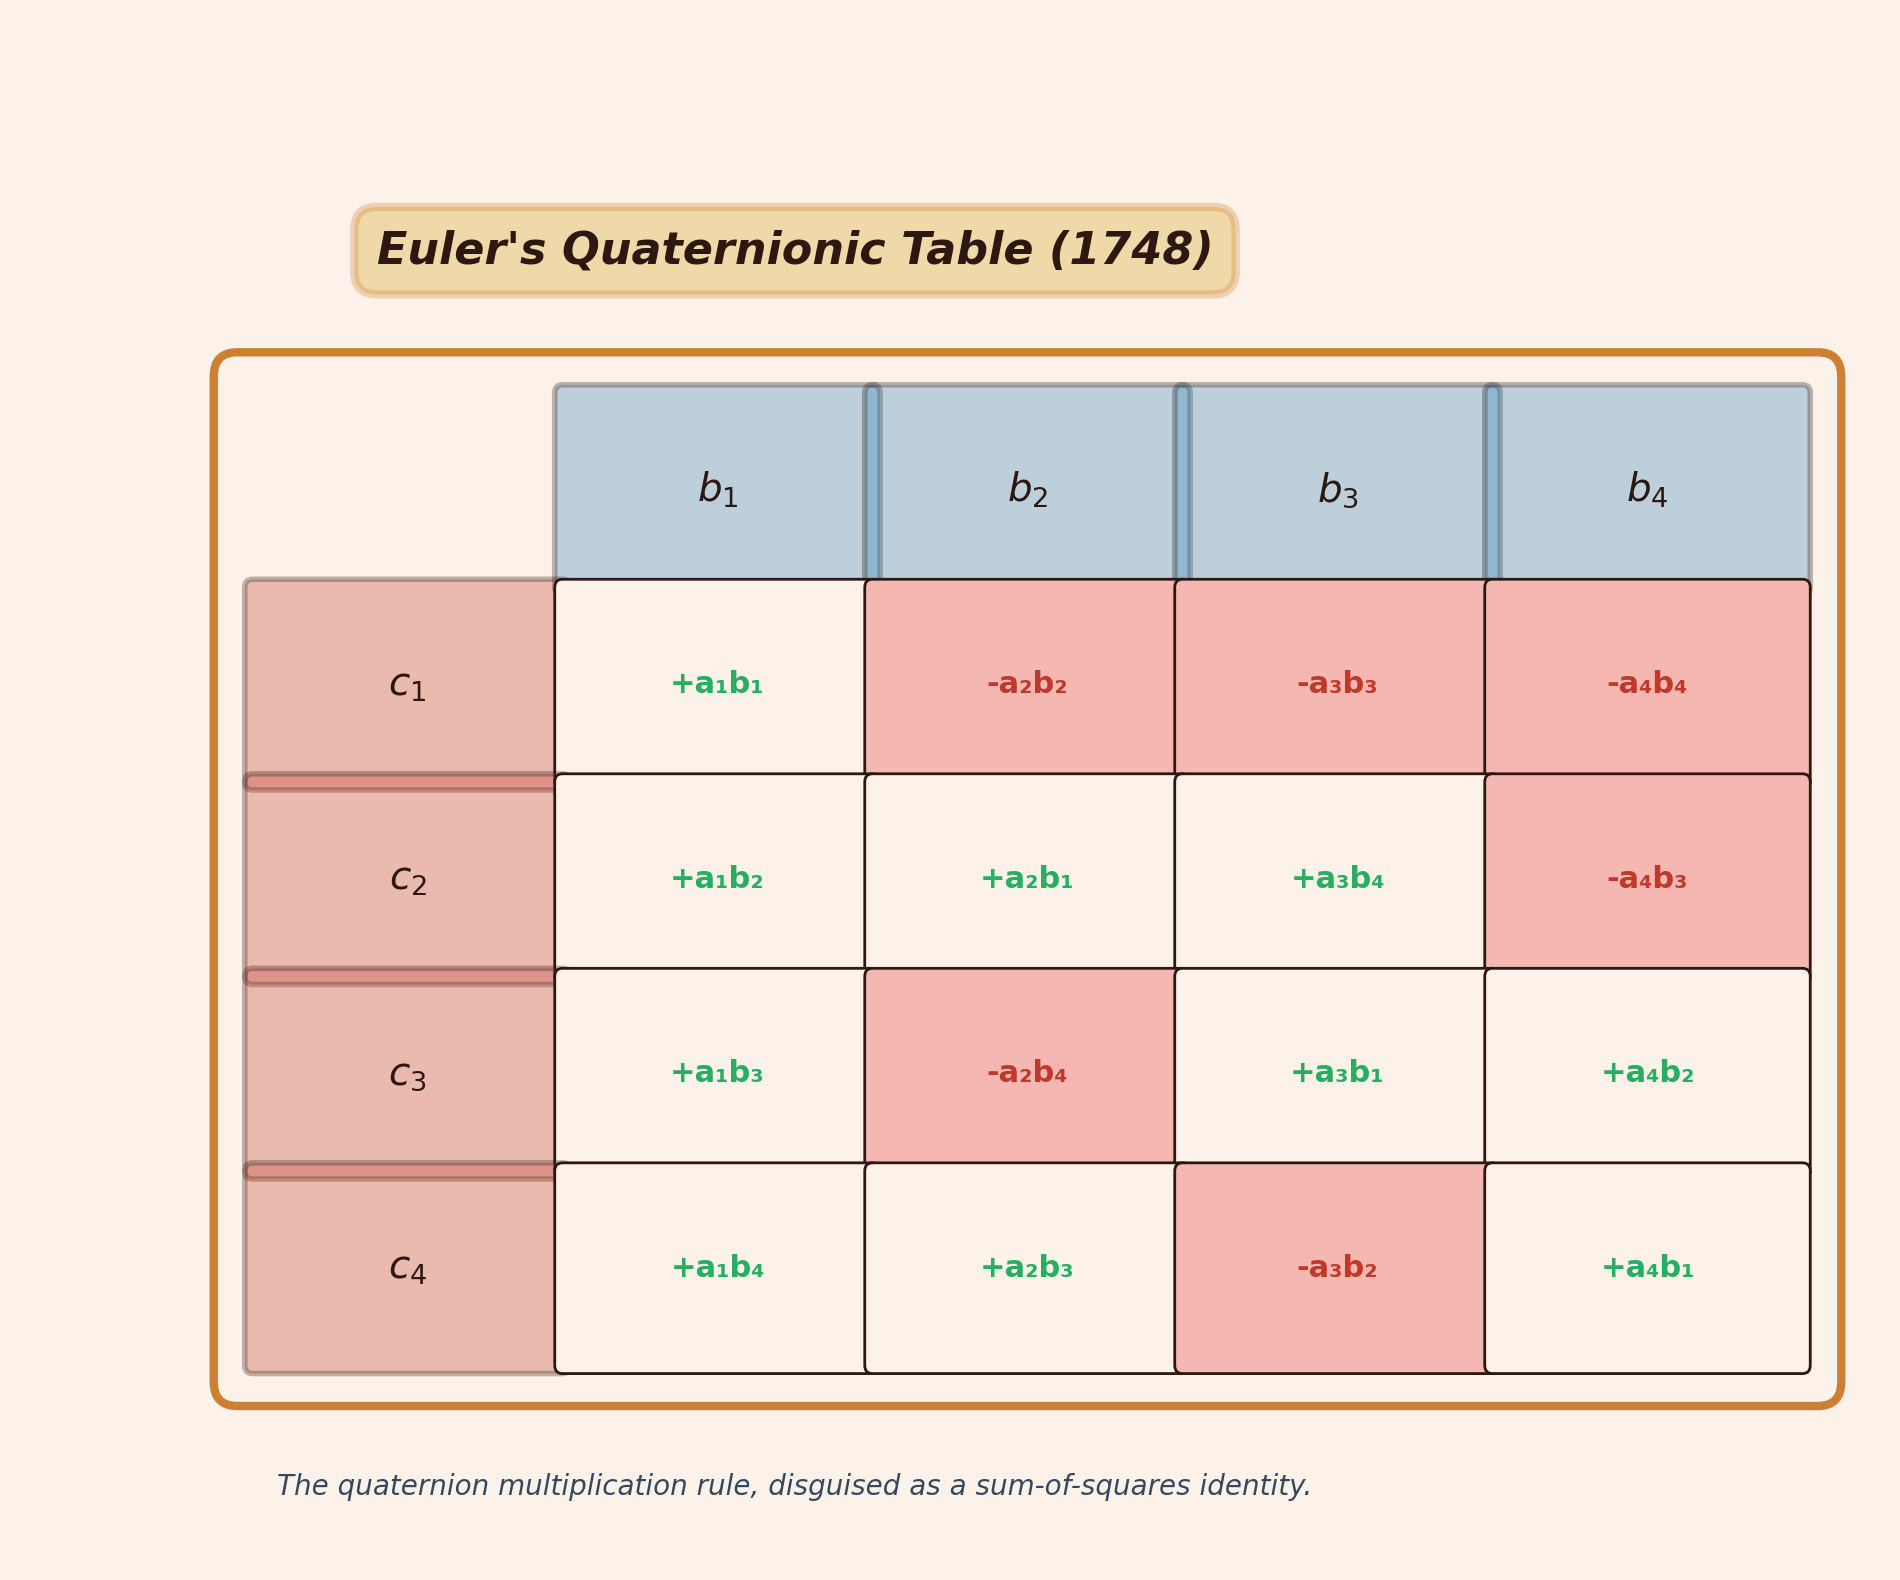
\includegraphics[width=0.82\textwidth]{../Chapter6/images/fig13_euler_table.png}
\end{figure}


Brahmagupta's \emph{Brāhmasphuṭasiddhānta} (628 AD) contained the two-square identity centuries before European mathematicians rediscovered it. Fibonacci popularized it in his \emph{Liber Quadratorum} (1225) --- ``The Book of Squares'' --- a masterpiece of medieval number theory that was almost entirely ignored by his contemporaries, who preferred his \emph{Liber Abaci} and the famous rabbit sequence. Euler proved the four-square version in 1748, and it was essential to Lagrange's 1770 proof that every positive integer is a sum of four squares.

The philosophical moral: these identities show that the world of sums of squares is \emph{closed under multiplication}. Products inherit the Pythagorean structure of their factors. And that closure is not an accident --- it is a shadow of the norm-multiplicativity of the normed division algebras: \(\mathbb{R}\), \(\mathbb{C}\), \(\mathbb{H}\) (the quaternions), and \(\mathbb{O}\) (the \index{octonions}octonions). Four algebras, four identities, four levels of the Pythagorean zoo. We are climbing the Cayley--Dickson tower --- and at every level, a new factoring tool awaits.



\section{Where All Roads Meet --- The Congruence of Squares}\label{ch6-where-all-roads-meet-the-congruence-of-squares}

Every modern factoring algorithm --- the \index{quadratic sieve}quadratic sieve, the \index{number field sieve}number field sieve, the algorithms that keep cryptographers awake at night --- ultimately rests on a single ancient trick: finding \(x\) and \(y\) such that

\[x^2 \equiv y^2 \pmod{N}\]

but \(x \not\equiv \pm y \pmod{N}\). When you have such a pair, the safe \emph{must} open. Let us see why, and then connect this grand unifying principle to everything we have built in this chapter.

\textbf{The Congruence of Squares Theorem.} Suppose \(N \mid (x^2 - y^2)\) but \(N \nmid (x - y)\) and \(N \nmid (x + y)\). Then:

\[1 < \gcd(x - y, \, N) < N.\]

The proof is almost too simple to be called a proof: since \(x^2 - y^2 = (x - y)(x + y)\) and \(N\) divides the product but neither factor alone, \(N\) must ``split'' across both factors. The GCD \(\gcd(x - y, N)\) captures whatever piece of \(N\) divides \(x - y\), and this piece is a nontrivial factor.

Now observe: every Pythagorean \(k\)-tuple with hypotenuse \(N\) gives rise to congruences of squares modulo \(N\). For each spatial component \(a_i\):

\[N^2 - a_i^2 = (N - a_i)(N + a_i) \equiv 0 \pmod{N}.\]

Since \(N \mid N^2\) and \(N \mid N^2 - a_i^2\), we have \(N \mid a_i^2\)\ldots{} no, wait --- let me be more careful. What we actually have is \(N^2 \equiv 0 \pmod{N}\), so \((N - a_i)(N + a_i) = N^2 - a_i^2\). But \(N - a_i\) and \(N + a_i\) are individually related to \(N\): \(\gcd(N - a_i, N)\) divides \(N\) automatically. The multi-channel theorem of Section 3 is, in retrospect, a systematic way of generating congruences of squares modulo \(N\) and extracting factors from them.

This is the grand unification. Fermat's factoring method (1643), Kraitchik's improvement (1920s), Morrison and Brillhart's continued-fraction method (1975), Pomerance's quadratic sieve (1981), and the Lenstra--Lenstra--Manassé--Pollard number field sieve (1993) --- all of these are, at their core, different strategies for finding congruences of squares. Our Pythagorean \(k\)-tuple machinery provides a \emph{systematic source} of such congruences, with the dimension \(k\) controlling how many you get from a single equation.

And here is the philosophical capstone, courtesy of Lagrange. By Lagrange's four-square theorem, every positive integer is a sum of four squares. Therefore, every integer \(N \geq 2\) can serve as the hypotenuse of at least one Pythagorean quintuplet (since if \(N^2 = a^2 + b^2 + c^2 + d^2\) for some \(a, b, c, d\), we have a quintuplet with hypotenuse \(N\)). Factoring channels are \emph{guaranteed to exist} for every composite number. The lock always has keyholes --- the question is only whether we can find the right keys.


\begin{figure}[htbp]
\centering
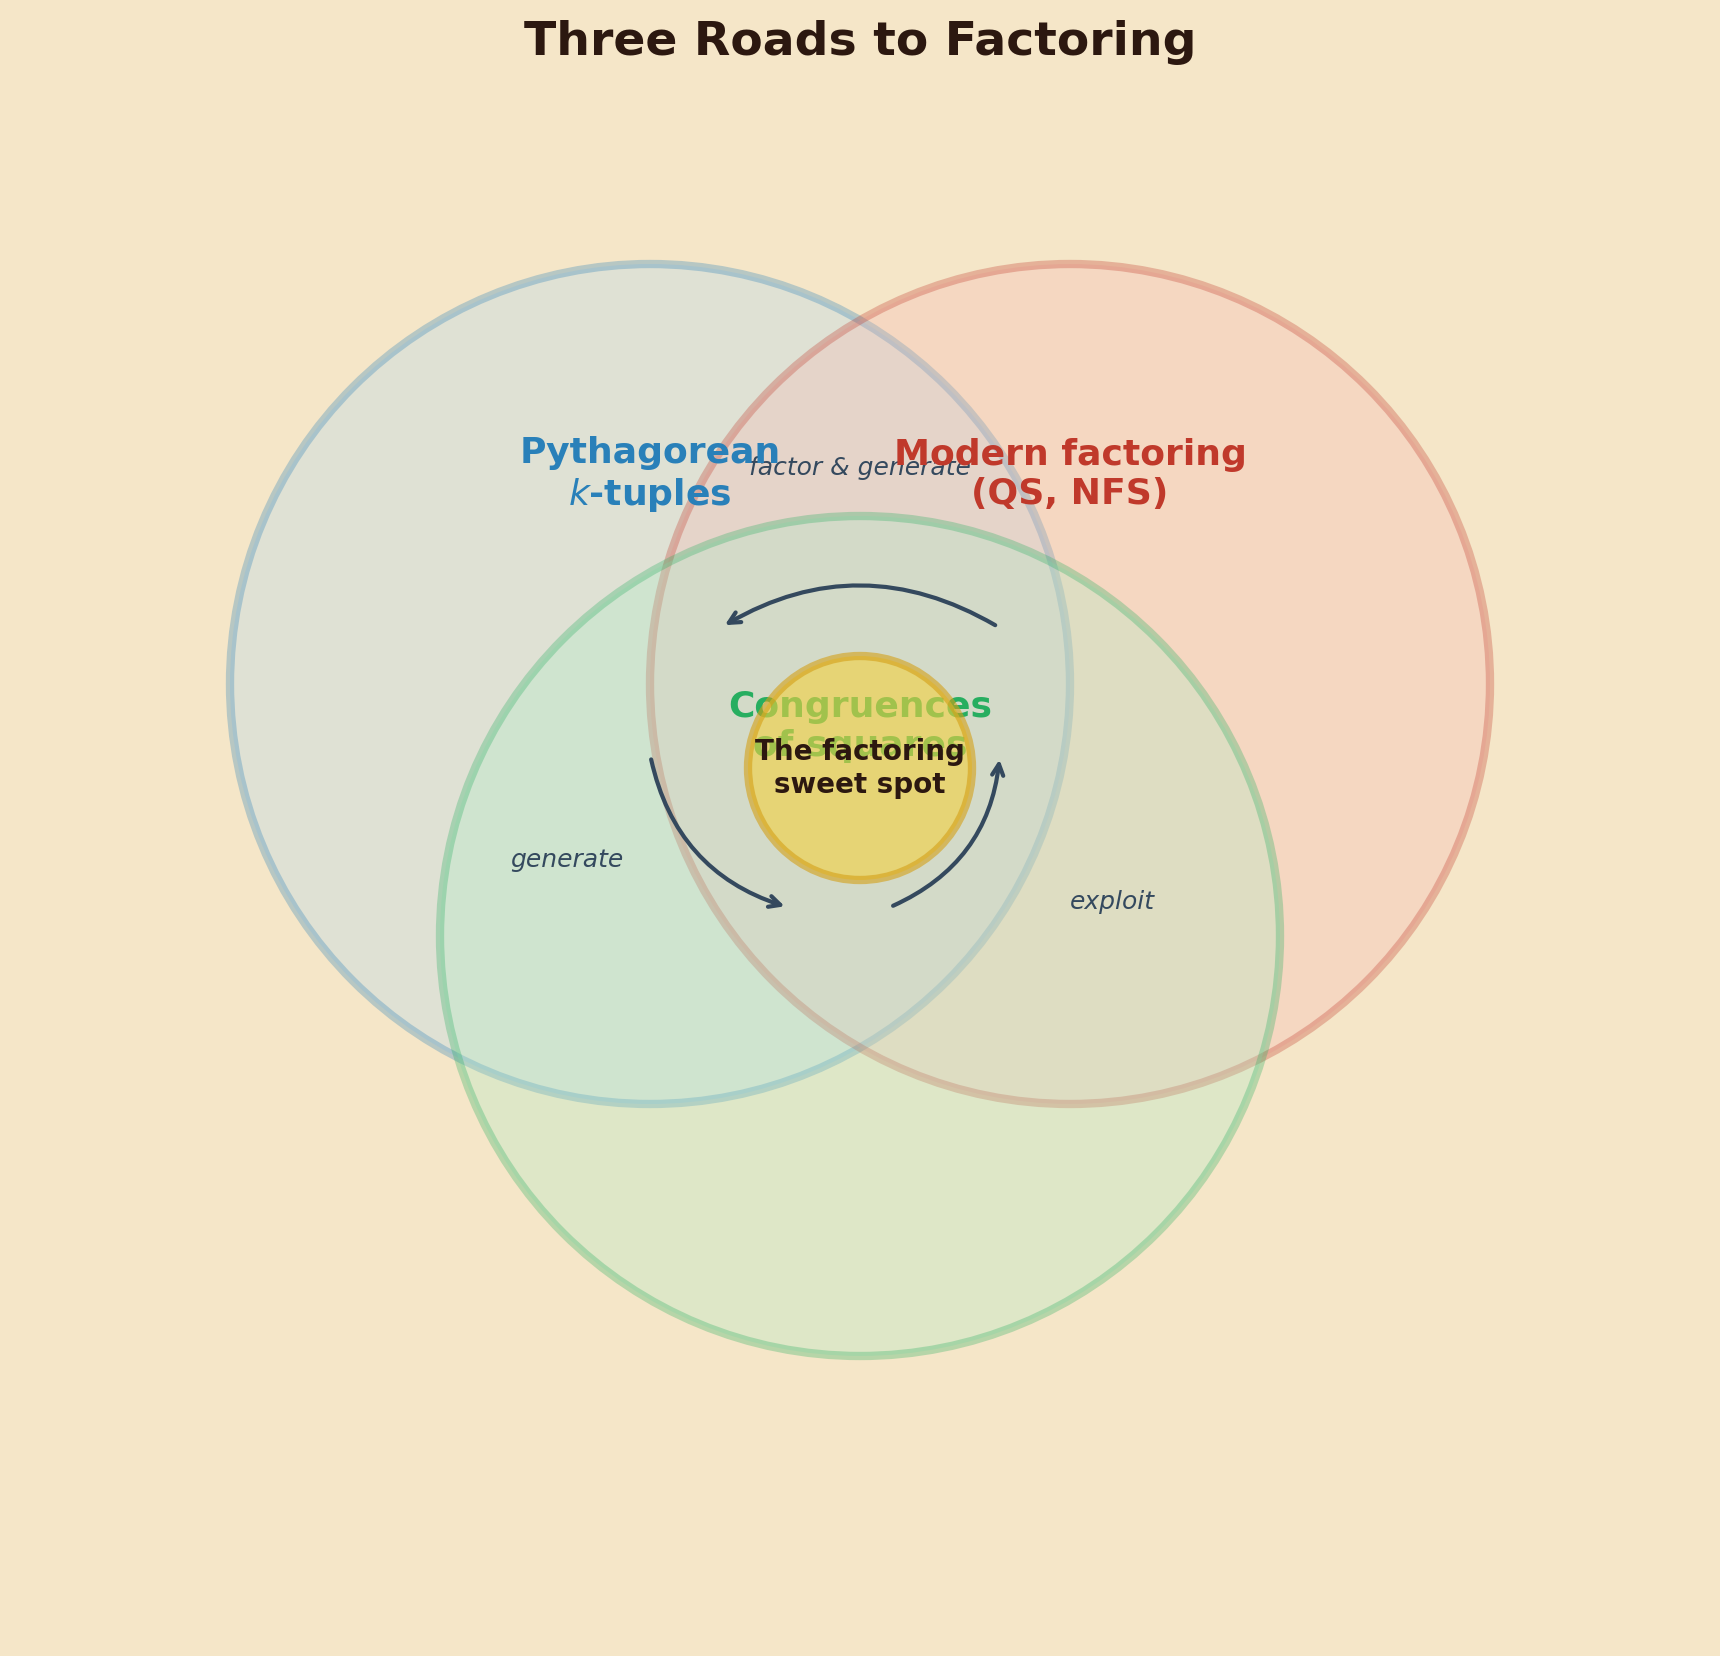
\includegraphics[width=0.82\textwidth]{../Chapter6/images/fig14_venn_diagram.png}
\end{figure}



\begin{figure}[htbp]
\centering
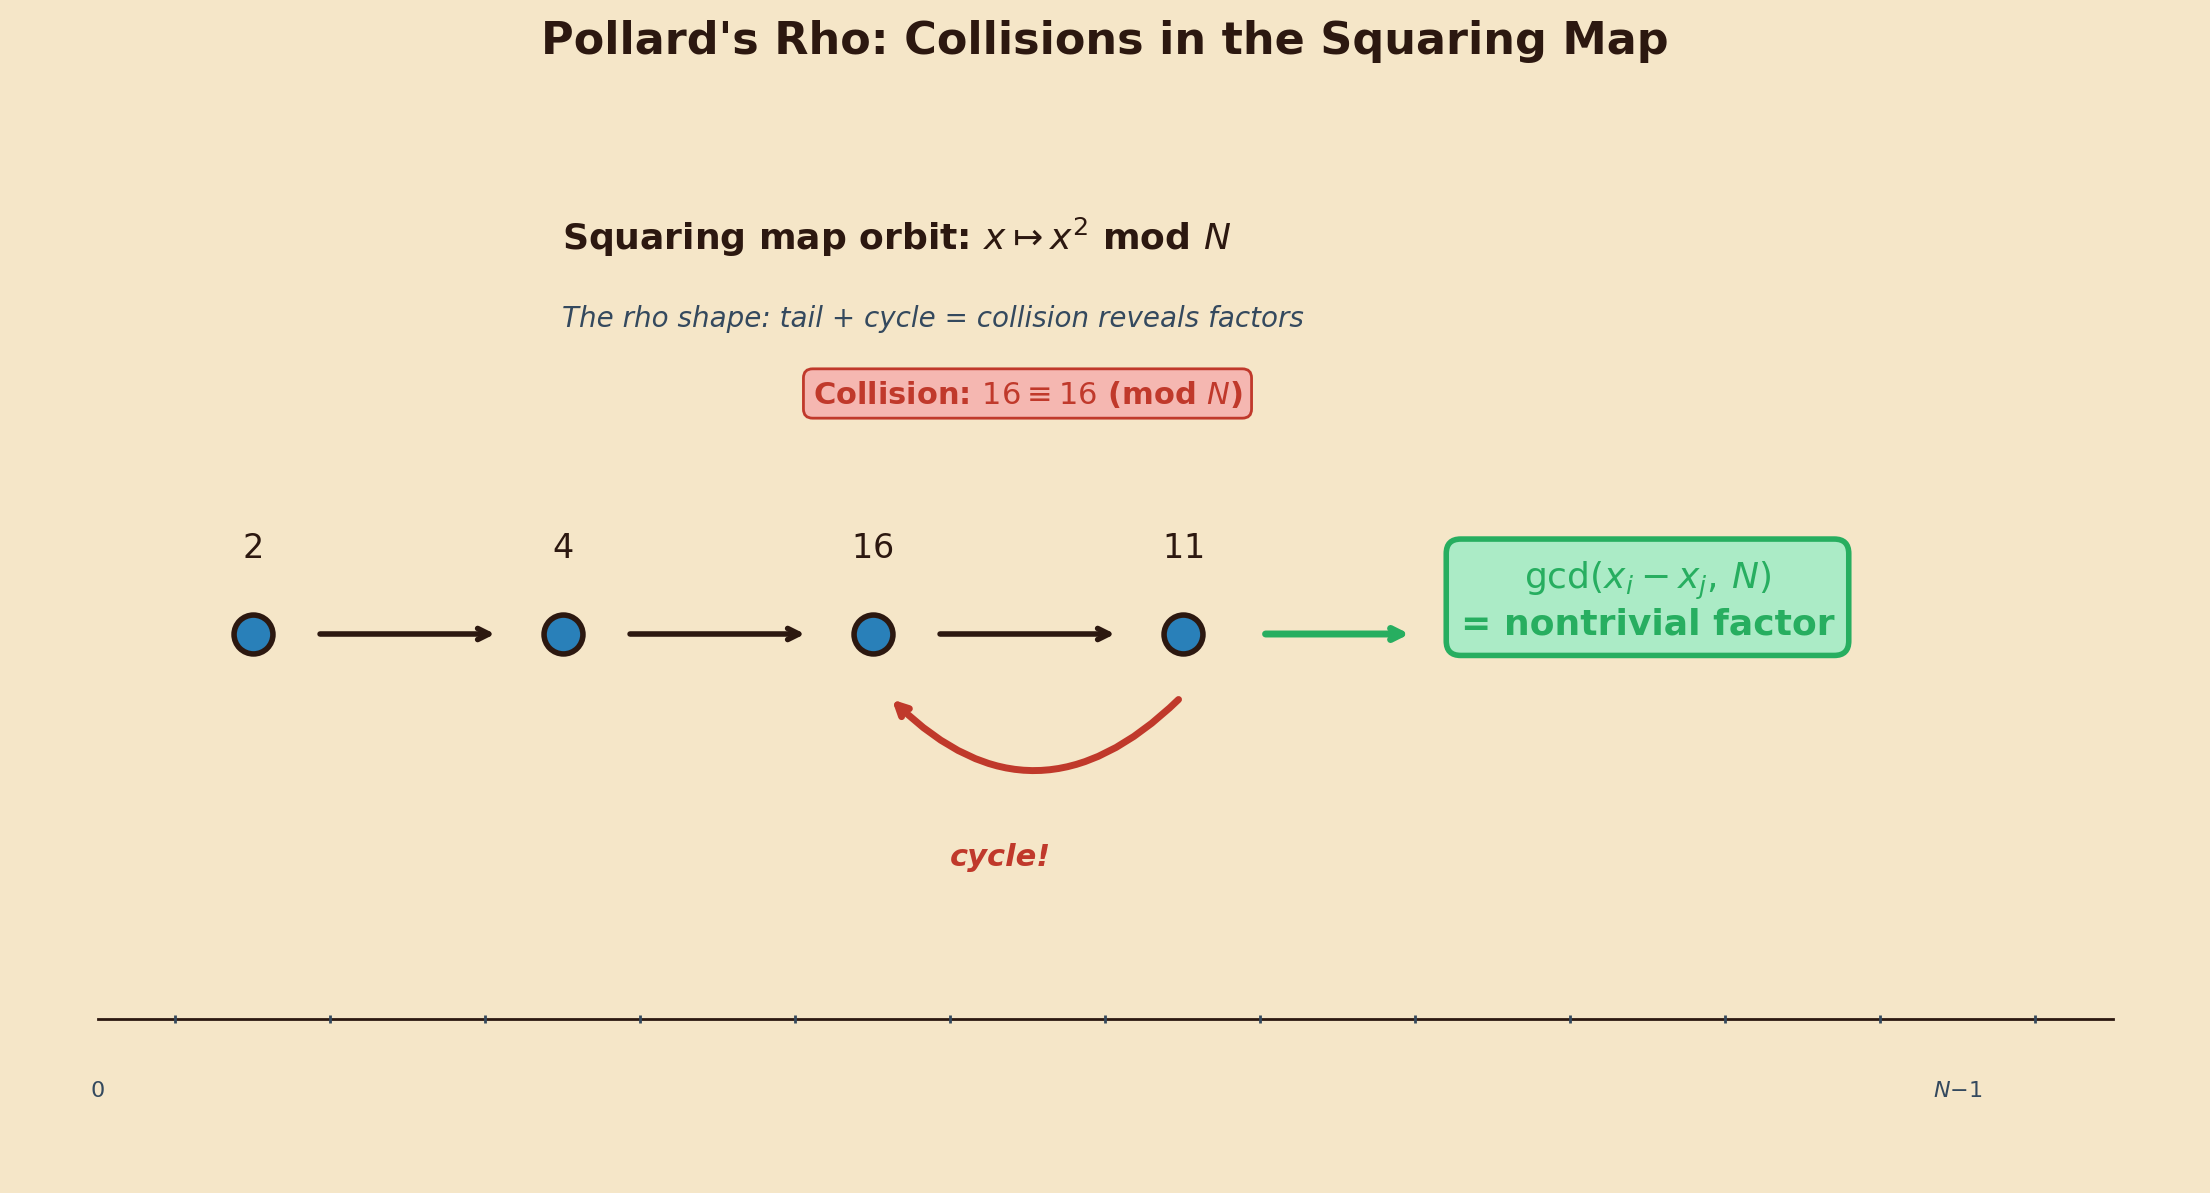
\includegraphics[width=0.82\textwidth]{../Chapter6/images/fig15_rho_orbit.png}
\end{figure}




\section{The Octopus's Garden --- A Meditation on Dimension and Difficulty}\label{ch6-the-octopuss-garden-a-meditation-on-dimension-and-difficulty}

If adding dimensions is so helpful, why not work in dimension \(1{,}000\)? A thousand spatial components would give \(\binom{1000}{2} + 1000 = 500{,}500\) factoring channels from a single equation. Surely that would crack any composite.

The answer is a lovely tension --- one of those trade-offs that mathematics delights in presenting just when you think you've found a free lunch. More channels make it \emph{easier to factor once you have a tuple}, but finding integer points on a high-dimensional null cone becomes \emph{harder in the wrong ways}. The sphere of radius \(N\) in \(\mathbb{R}^k\) has surface area proportional to \(N^{k-1}\), and the density of integer lattice points on it follows subtle laws governed by the theory of modular forms and theta functions.

The key player is Jacobi's theta function \(\vartheta(q) = \sum_{n=-\infty}^{\infty} q^{n^2}\), whose \(k\)-th power counts the number of representations \(r_k(n)\) --- the number of ways to write \(n\) as a sum of \(k\) squares (counting signs and ordering). For \(k = 4\), Jacobi gave the exact and beautiful formula:

\[r_4(n) = 8 \sum_{\substack{d \mid n \\ 4 \nmid d}} d.\]

This tells us that \(r_4(n)\) grows roughly like \(n\) itself (the sum of divisors), so representations as sums of four squares are abundant. But we need more than abundance --- we need a representation where the sum is a \emph{perfect square}, \(N^2\). And the number of such representations is a subtler quantity, controlled by the arithmetic of \(N\) in ways that do not simplify as cleanly.

The philosophical point is this: the difficulty of factoring is \emph{not} in finding channels, but in finding the right Pythagorean representation. The \(k\)-tuple framework \emph{redistributes} the difficulty --- it does not eliminate it. In low dimensions, representations are scarce but channels are few. In high dimensions, channels are plentiful but representations are harder to find. The sweet spot --- the dimension where the product of ``ease of finding a tuple'' and ``number of channels per tuple'' is maximized --- is a fascinating open question that connects number theory to optimization, lattice geometry, and the physics of sphere packings.

There is one more thread to pull, and it leads to the deepest waters in algebra. The Brahmagupta--Fibonacci identity (two squares), the Euler four-square identity (four squares), and the Degen--Graves eight-square identity (eight squares) correspond to the four normed division algebras: the real numbers \(\mathbb{R}\), the complex numbers \(\mathbb{C}\), the quaternions \(\mathbb{H}\), and the octonions \(\mathbb{O}\). These are the \emph{only} dimensions --- \(1, 2, 4, 8\) --- in which a multiplicative sum-of-squares identity exists. This is the Hurwitz theorem (1898), and it is one of the most remarkable rigidity results in all of mathematics.

At each step up the Cayley--Dickson construction --- reals to complex, complex to quaternions, quaternions to octonions --- an algebraic property is lost: first ordering, then commutativity, then associativity. The octonions are the last stop; beyond them lie the sedenions, which lose the division property and with it the sum-of-squares identity. The ``cost'' of higher-dimensional factoring is paid in algebraic structure: the more powerful the identity, the less well-behaved the algebra.

And so we arrive back at our octopus, with its seven tentacles and its twenty-eight channels, sitting contentedly in a garden of numbers. The octopus lives in dimension eight --- the last dimension where the algebra is clean, where the multiplication identity holds, where factoring channels compose nicely. It is the perfect creature for the job: not too small to be weak, not too large to be unwieldy. Seven keyholes, twenty-eight keys, one ancient equation --- and behind the door, the prime factors of \(N\), waiting to be found.


\begin{figure}[htbp]
\centering
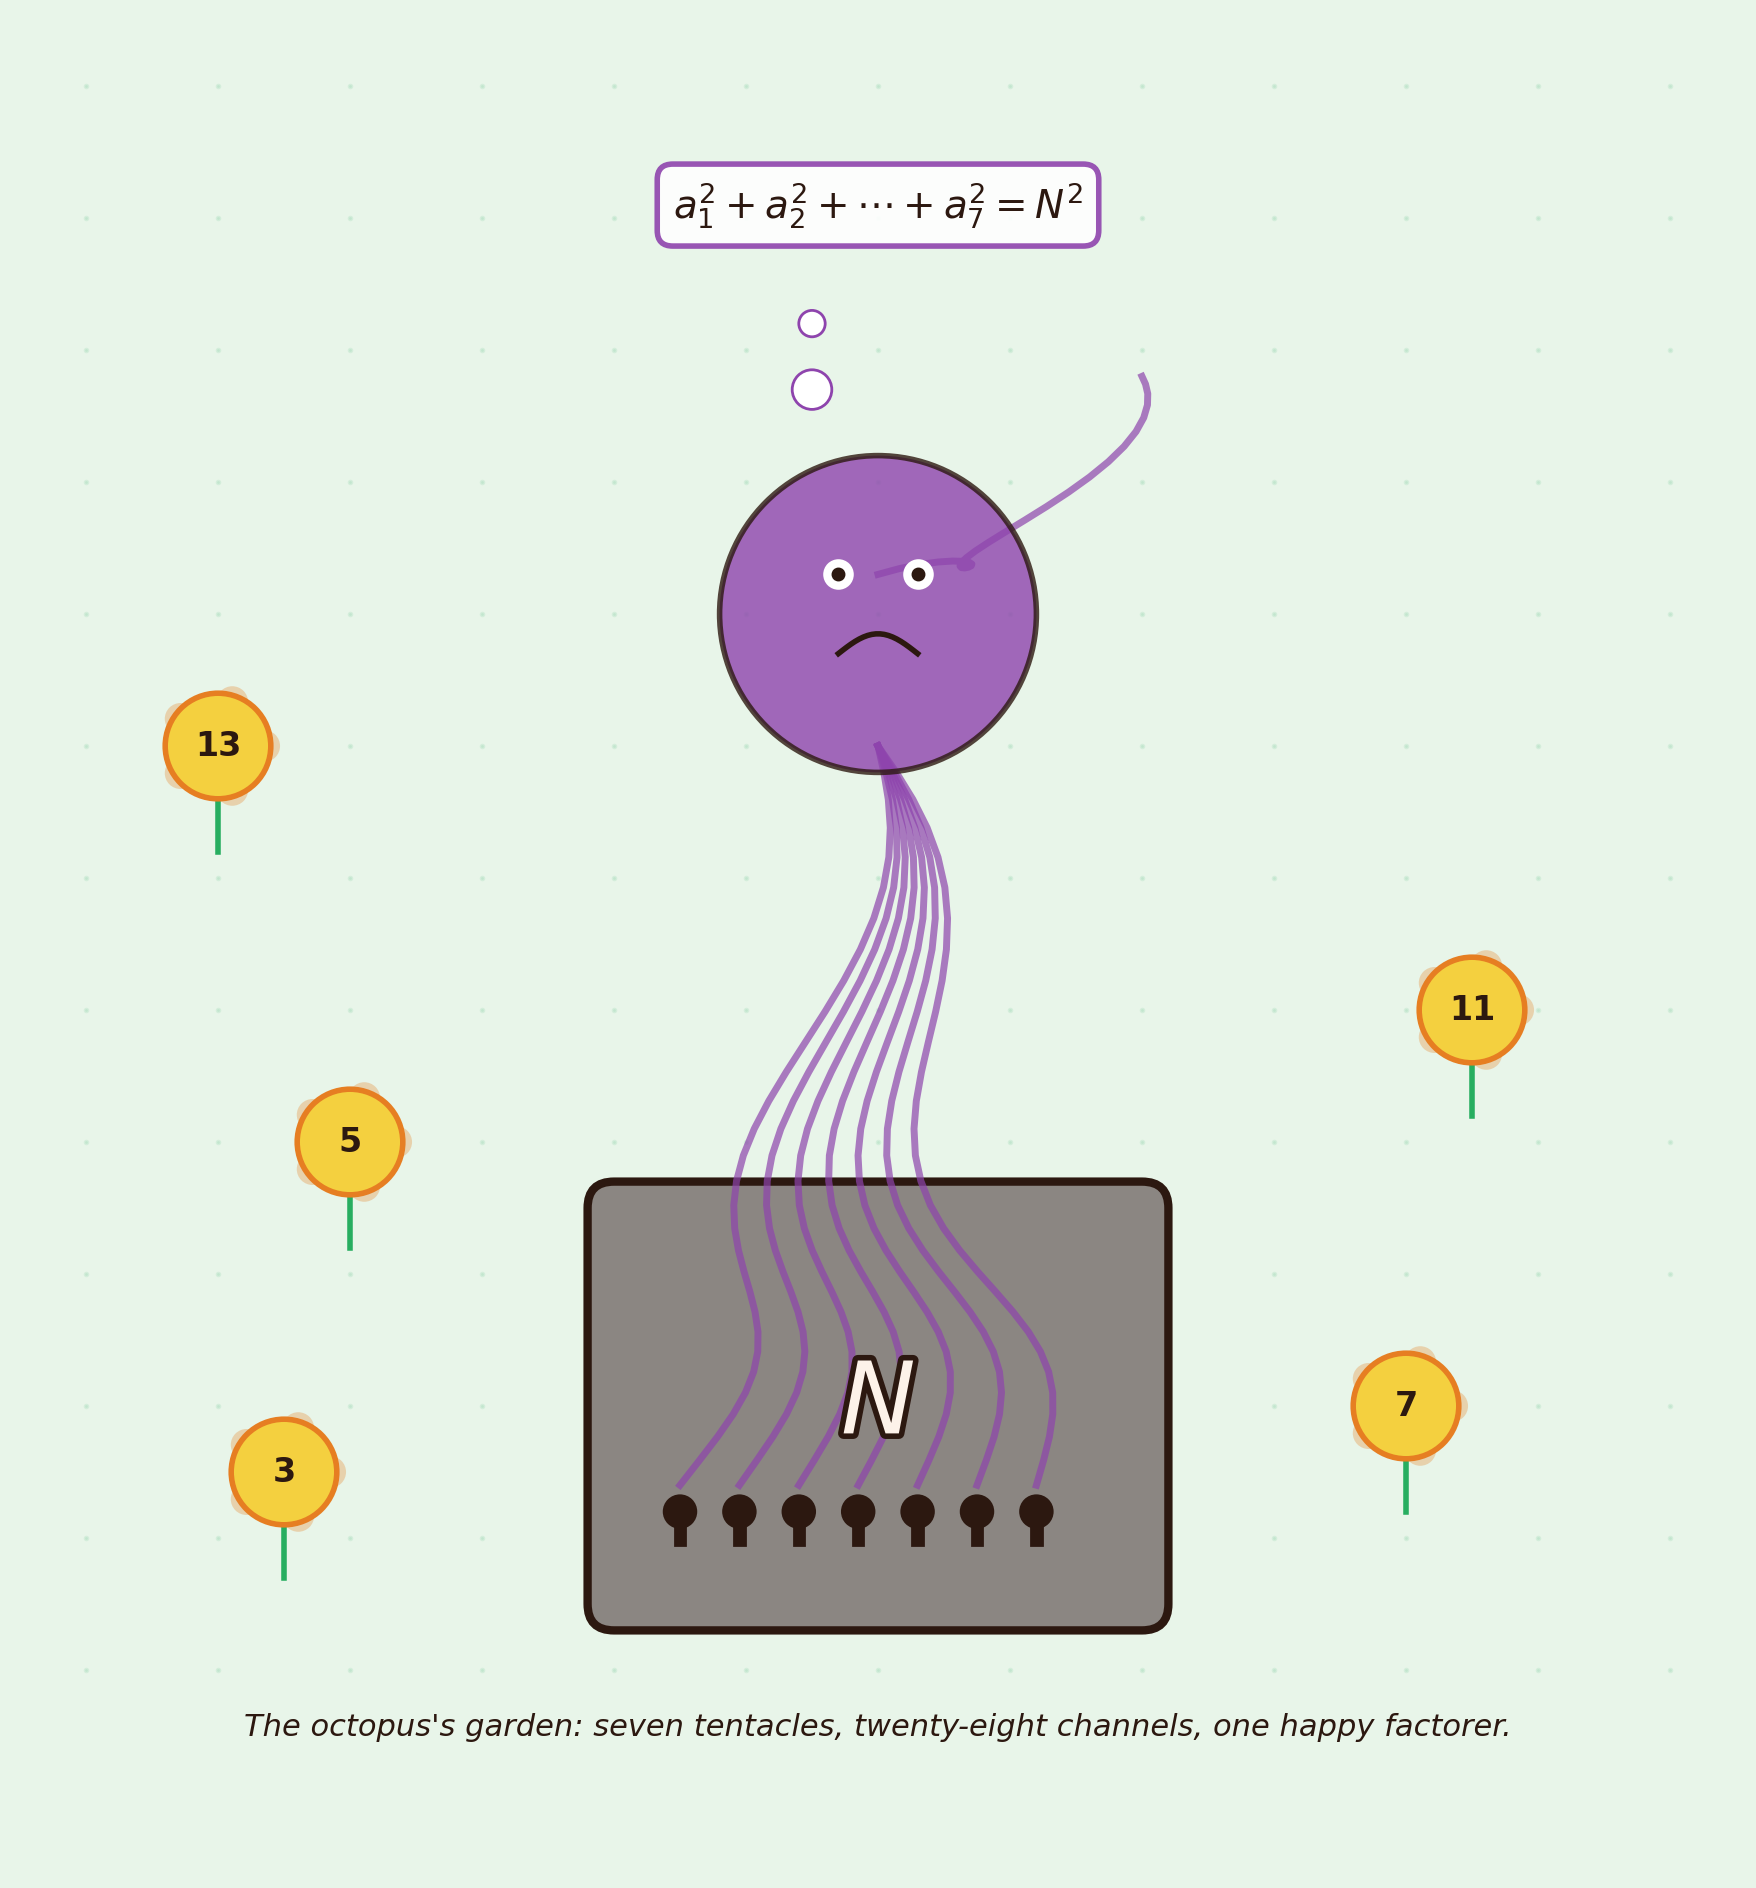
\includegraphics[width=0.82\textwidth]{../Chapter6/images/fig16_octopus_garden.png}
\end{figure}




\section{Exercises}\label{ch6-exercises}

\begin{enumerate}
\def\labelenumi{\arabic{enumi}.}
\item
  \textbf{(The Quintuplet Zoo)} Find a Pythagorean quintuplet \((a, b, c, d, e)\) where all four spatial components \(a, b, c, d\) are distinct primes. \emph{(Hint: try the four smallest odd primes.)}
\item
  \textbf{(Cracking 77)} Find a Pythagorean quadruple \((a, b, c, 77)\) with hypotenuse \(77\), and use the multi-channel theorem to extract a nontrivial factor of \(77\).
\item
  \textbf{(The Octuplet Census)} For the octuplet \((1, 2, 3, 4, 5, 6, 3, 10)\), compute all seven primary GCDs \(\gcd(10 - a_i, 10)\). Which ones yield nontrivial factors of \(10\)?
\item
  \textbf{(Inside-Out at 35)} For \(N = 35\), find integers \(u, v\) such that \(35^2 + u^2 + v^2\) is a perfect square. \emph{(Hint: try small values of \(u\) and \(v\) systematically.)}
\item
  \textbf{(Berggren Descent)} Apply \(B_2^{-1}(a, b, c) = (a + 2b - 2c,\; 2a + b - 2c,\; -2a - 2b + 3c)\) to the triple \((5, 12, 13)\) and verify that the parent is a Pythagorean triple with a smaller hypotenuse.
\item
  \textbf{(Mirror, Mirror)} Apply \(R_{1111}\) to the quadruple \((5, 10, 10, 15)\). Verify the reflection is Pythagorean. Find all three GCD channels for \(N = 15\).
\item
  \textbf{(Brahmagupta's Gift)} Use the Brahmagupta--Fibonacci identity to write \(65 = 5 \times 13\) as a sum of two squares in \emph{two} different ways. \emph{(Hint: \(5 = 1^2 + 2^2\) and \(13 = 2^2 + 3^2\); now try both sign choices in \((ac \mp bd, \, ad \pm bc)\).)}
\item
  \textbf{(The Congruence of Squares)} Find integers \(x, y\) with \(x^2 \equiv y^2 \pmod{21}\) but \(x \not\equiv \pm y \pmod{21}\), and use the \index{congruence of squares}congruence of squares theorem to extract a factor of \(21\).
\end{enumerate}
